%%%%%%%%%%% prima parte del corso - Mobile Computing %%%%%%%%%%% 
\chapter{Introduzione al Mobile Computing - Mobile Computing}
\lhead{Introduzione al Mobile Computing - Mobile Computing}
\rhead{Lezione 1 - 30 settembre}
\begin{center}
    \textbf{--------- Lezione 1 - 1 marzo 2021 ---------}
\end{center}

\section{Concetti preliminari}
\subsection{Calcolo della posizione indoor vs outdoor}
La maggior parte delle app richiede una maggior precisione, l'altezza infatti è fondamentale: sono al primo o al quinto piano di un edificio?
Negli ambienti outdoor l'altezza non è così fondamentale.

Le tecniche che utilizziamo in outdoor non possono essere utilizzate in indoor:
\begin{itemize}
    \item GPS: linea di comunicazione tra la sorgente (satellite) e il dispositivo
    \item le interferenze possono rendere inutilizzabile il sistema segnale, come il segnale radio che viene disturbato da muri o da altri ostacoli
\end{itemize}  

L'area di copertura in indoor è ridotta. 
Nel maggior parte dei casi lo spostamento avviene a piedi ed il vantaggio spostandosi lentamente è che si ha una minore rapidità di spostamento degli utenti, lo svantaggio è che siamo soggetti a rumori come a cambiamenti di direzione improvvisi. 

Attualmente l'indoor positioning è ancor poco comune.

\textit{\textbf{Chi è il soggetto da localizzare?}}
\\ Possiamo voler monitorare la posizione di persone, robot o oggetti come ad esempio il carrello delle emergenze in un ospedale. 
\\ Soggetti diversi implicano tecnologie diverse:
\begin{itemize}
    \item per le persone abbiamo tecniche di posizionamento che sfruttano i dispositivi mobili degli utenti
    \item per i robot e gli oggetti possiamo prevedere un hardware apposito
\end{itemize}

\textit{\textbf{Chi effettua il calcolo della posizione?}} 
\\ Ci sono due tipi di tecniche: 
\begin{itemize}
    \item tecniche attive: il calcolo della posizione viene effettuato dal dispositivo in movimento (le tecniche trattate nel corso)
    \item tecniche passive: l'hardware distribuito nell'ambiente capisce in che posizione sono gli utenti 
\end{itemize}

\subsection{Applicazioni principali}
\begin{itemize}
    \item navigazione: non è una tecnologia molto utilizzata. Sapere dove muovermi all'interno di un aeroporto sarebbe comodo, come ad esempio "guidami fino al gate 15"
    \item location based services: vengono utilizzati per l'outdoor, non ancora per l'indoor 
    \item home automation: es. un sistema che in base alla stanza nel quale mi sposto, accende le luci
    \item context detection: es. il riconoscimento precoce di malattie degenerative tramite un'analisi del comportamento degli utenti
    \item social networking: es. friend finder
    \item emergenze: es. in caso di incendio i vigili del fuoco sanno dove sono le persone da salvare
\end{itemize}

\subsection{Paradigmi di navigazione}
\begin{itemize}
    \item Navigazione allocentrica: il sistema fornisce le indicazioni di navigazione rispetto all'ambiente come ad esempio la vista dall'alto con la mappa. 
    \item Navigazione egocentrica: il sistema fornisce le indicazioni di navigazione rispetto all'utente, come ad esempio una freccia che indica dove andare
\end{itemize}
L'interpretazione da parte dell'utente delle informazioni allocentriche richiede all'utente di conoscere com'è orientato e non sempre questa navigazione è possibile quando c'è ad esempio del fumo o della nebbia. 

\subsection{Caratteristiche dei sistemi di posizionamento indoor}
Quali caratteristiche deve avere il sistema per adattarsi alle necessità dell'utente?
\begin{itemize}
    \item il sistema indoor deve essere preciso nel calcolo della posizione
    \item area di copertura (stanza, edificio, globale)
    \item il costo (di installazione, di manutenzione, ecc.)
    \item infrastruttura (nessuna, trasmettitori sparsi nell'ambiente, ecc.)
    \item maturità della tecnologia (prototipo, prodotto, ecc.)
    \item tipo di informazione di posizione che viene prodotto (posizione 2D/3D, orientamento, ecc)
    \item privacy (il sistema viene a sapere dove si trova l'utente?)
    \item frequenza di update (quando l'utente fa qualcosa, automatico ogni 4 secondi)
    \item azione richiesta all’utente (nessuna, inquadrare il marker, ecc.)
    \item interfaccia (grafica, vocale, ecc.)
    \item robustezza della misura (nelle giornate affollate, ecc.)
    \item robustezza della sistema (i beacon si possono rubare, i marcatori si staccano, ecc.)
    \item scalabilità (non scalabile, scalabile aumentando l’infrastruttura, scalabile diminuendo l’accuratezza, ecc.)
    \item impatto sull'ambiente (i marcatori visivi rovinano l’aspetto estetico, ecc.)
\end{itemize}

\section{Tecniche di posizionamento}
Ci sono 4 tecniche di posizionamento indoor che verranno approfondite:
\begin{itemize}
    \item immagini
    \item segnali radio
    \item sistemi inerziali
    \item soluzioni ibride
\end{itemize}

\section{Tecniche basate su immagini}
Ci sono diverse tecniche che permettono di calcolare la posizione usando le immagini tra cui i marcatori visivi.
I marcatori visivi sono oggetti facilmente riconoscibili tramite tecniche di computer vision. Distinguiamo marcatori:
\begin{itemize}
    \item espliciti: progettati per essere facilmente riconoscibili come i QR-code
    \item impliciti: creati per altri scopi, ma facilmente riconoscibili con tecniche di computer vision come i cartelli stradali
\end{itemize}

I marcatori visivi possono essere installati nell'ambiente. Quando un utente ad esempio inquadra il marcatore, so che l'utente si trova lì vicino. Ciascun marcatore contiene la propria posizione oppure un identificatore che il device sa associare alla posizione. 

\subsection{Pro e contro dei marcatori espliciti}
\begin{table}[!ht]
    \centering
    \begin{tabular}{p{.45\textwidth}|p{.45\textwidth}}
        \textbf{Vantaggi} & \textbf{Svantaggi} \\
        \hline
        \begin{itemize}
            \item tecnologia semplice e stabile 
            \item i marcatori sono economici
        \end{itemize} & 
        \begin{itemize}
            \item la precisione è legata alla distanza alla quale il device riesce a riconoscere il marcatore
            \item non permettono di calcolare l'angolo
            \item è richiesta un'azione esplicita all'utente
        \end{itemize}
    \end{tabular}
\end{table}

\subsection{I marcatori impliciti}
Se so la dimensione in centimetri del marcatore, dove viene appeso e con che angolo, quando il marcatore viene inquadrato, posso usare tecniche di geometria per capire dove si trova l'utente rispetto al marcatore. 

Però ho un problema: ho il sistema dove ho cartelli facilmente riconoscibili e sviluppo una tecnica che riconosca i cartelli ma ci potrebbero essere due cartelli uguali. 
Bisogna combinare la tecnica con altre tecniche ad esempio usando i segnali radio. 
La tecnica funziona da sola nel caso in cui i marcatori impliciti siano tutti diversi. 

\subsubsection{Pro e contro}
\begin{table}[!ht]
    \centering
    \begin{tabular}{p{.45\textwidth}|p{.45\textwidth}}
        \textbf{Vantaggi} & \textbf{Svantaggi} \\
        \hline
        Non devo installare altri segnali nell'ambiente (in alcuni ambienti potrebbe essere impossibile, ad esempio nei musei) & se i marcatori non sono univoci la tecnica da sola non permette di calcolare la posizione e deve essere combinata con altre tecniche
    \end{tabular}
\end{table}

\subsubsection{Tecniche marker-less}
Per risolvere i problemi posso usare tecniche marker-less, non vengono scelti marcatori da me programmatore ma il sistema estrae da solo delle informazioni visive che permettono poi all'utente di capire dove si trova.
Questa tecnica opera a due fasi:
\begin{itemize}
    \item setup: viene costruita una mappa 3D dell'ambiente, il sistema identifica diversi punti di riferimento con caratteristiche geometriche peculiari
    \item calcolo posizione: quando l'utente è nell'ambiente, vengono identificati alcuni punti di riferimento e poi vengono confrontati con quelli ottenuti in fase di setup, per risalire alla posizione
\end{itemize}

Ho però un problema: durante la fase di setup ho un dispositivo che mentre si muove, deve creare una mappa dell'ambiente e deve sapere dove sono rispetto all'ambiente. 

Durante la fasi di calcolo della posizione, dal device mobile si cerca di trovare gli stessi punti di riferimento identificati in fase di setup e di stimare la posizione della camera rispetto ad essi. 

Ho un problema: due zone possono avere le stesse caratteristiche, ad esempio possono esserci due stanze che presentano le stesse feature su piani diversi di un edificio.



\chapter{Sistemi operativi}
\lhead{Sistemi operativi - Mobile Computing}
\rhead{Lezione 2 - 2 ottobre}
\begin{center}
    \textbf{--------- Lezione 2 - 4 marzo 2021 ---------}
\end{center}
\subsection{Uso di tecniche di visione per posizione outdoor}
Dalle immagini catturate dalla macchina google (street view) possiamo estrarre dei punti di riferimento (feature points). 
La posizione da cui sono scattate le foto stradali è nota con buona precisione, quindi si riesce a conoscere la posizione dei feature points.
\\ Quando l'utente inquadra attorno a sé, si conosce più o meno la posizione, e dalle immagini dell'utente si identificato le feature che corrispondono a quelle identificate dalle immagini stradali. Poi si fa un match con i feature points della macchina google in modo tale che si possa calcolare la posizione dell'utente rispetto alla macchina (dato che so come si trova la macchina rispetto ai feature points).
Si calcola la posizione (molto precisa) e l'orientamente dell'utente. 

Una funzione simile è messa a disposizione per le librerie AR da Apple (ARKit).    

\section{Calcolo della posizione basato su segnale radio}
I dispositivi mobili al momento sono dotati di hardware per questi segnali radio:
\begin{itemize}
    \item WiFi: abbiamo un problema applicativo, con le tecnologie attuali non è possibile da programma accedere alle antenne WiFi nelle vicinanze, il SO operativo conosce le informazioni ma le API dei dispositivi iOS non consentono al programmatore di accedere. 
    \item bluetooth: dispositivi detti beacon da acquistare ed installare specificamente per il calcolo della posizione
    \item Near Field Communication (NFC)
    \item Ultra Wide-Band (UWB): ancora poco diffuso nei dispositivi mobili
\end{itemize}
RSSI indica la potenza del segnale ricevuto dal dispositivo mobile. 

Ci sono 3 diverse tecniche basate su segnale radio:
\begin{itemize}
    \item prossimità
    \item multilaterazione
    \item fingerprinting
\end{itemize}

\subsection{Posizionamento per prossimità}
Il dispositivo mobile percepisce il segnale radio inviato da un'antenna con un certo identificativo. 
Se conosciamo l'id dell'antenna e la distanza massima con la quale si può percepire il segnale da quell'antenna, allora riusciamo a scoprire la posizione di un device. 

L'accuratezza con Wifi e bluetooth è bassa mentre con NFC è alta ma il calcolo della posizione avviene solo quando l'utente avvicina il device ad un sensore NFC installato nell'ambiente.

Ci sono due limiti parlando di prossimità:
\begin{itemize}
    \item si considera una sola antenna
    \item si considera solo il fatto di percepire il segnale di quell'antenna, non si prova a stimare la distanza dall'antenna stessa
\end{itemize} 

\subsection{Multilaterazione}
Posso sapere che sono vicino ad un'antenna senza sapere la distanza oppure posso provare a stimare la distanza usando RSSI ma mi aspetto che la potenza decresca con l'aumentare della distanza.

\subsubsection{Calcolo della distanza con RSSI}
Conosciamo la potenza del segnale inviato, le caratteristiche dell'antenna, vogliamo calcolare la distanza ma abbiamo un altro fattore da prendere in considerazione che non conosciamo, il path lost factor che dipende dall'ambiente (è un fattore di attenuazione del segnale). 
\\ In ambienti aperti assume un valore di 2, in ambienti indoor tra 4 e 6 e in particolari indoor ha un valore minore di 2. 
\\ Stimando con RSSI si ottengono errori troppo grandi.
\\ Una tecnica per risolvere il problema è utilizzare un WiFi Round Trip Time.
\\ Google ha proposto una soluzione basata su RTT. 
RTT è la misura che rappresenta quanto ci mette un segnale ad andare e tornare da un'antenna. 

\subsection{Fingerprinting (o "scene analysis")}
La soluzione più adottata per risolvere i problema della multilaterazione è quella del fingerprinting.
Il valore di un RSSI in un punto è più o meno sempre quello, ma se metto più antenne, è difficile che la combinazione di questi valori si ripeta in un altro punto.

Data una posizione, il fingerprint è l’insieme di coppie $<$ID, RSSI\_ID$>$ dove ID è l’identificatore di un’antenna e RSSI\_ID il suo valore di RSSI misurato nella data posizione.

Un addetto si sposta all'interno dell'edificio segnalando al sistema la posizione corrente (es: toccando con il dito sulla mappa) e poi misura la potenza del segnale.
Questa operazione viene ripetuta in tutto l'ambiente, ad esempio ogni metro e prende le misure per tutte le antenne del fingerprint. 
\\ Il risultato prende il nome di radio map. 

La radio map contiene un insieme di coppie \textbf{$<$posizione, fingerprint$>$}, quindi \textbf{$<$posizione, [$<$ID, RSSI\_ID$>$]$>$}.

Quando un utente si trova nell'ambiente e vuole calcolare la posizione, possiamo prendere il fingerprint nella posizione corrente. 

Il modo più semplice per trovare la posizione dell'utente è: 
\begin{itemize}
    \item considerare tutti fingerprint in tutte le posizioni della radio-map
    \item calcolare il fingerprint dell'utente
    \item calcolare la distanza dal fingerprint in radio map
    \item vedere a quale campione l'utente è più vicino e assumo che quel campione sia la sua posizione
\end{itemize}


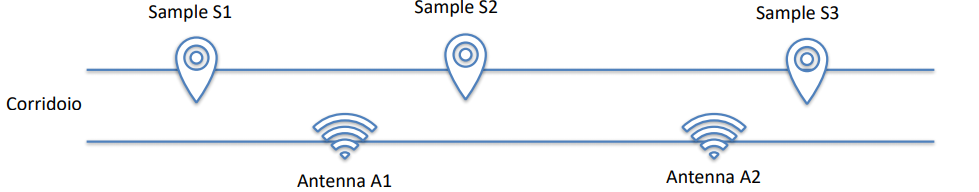
\includegraphics[width = \textwidth]{images/MobiDEV/1. posizionamento indoor/fingerprinting 1.PNG}

Ad esempio ho un corridoio con due antenne e riesco a percepirne sempre il segnale. Un incaricato misura i fingerprint in 3 posizioni campione e misura su ognuna la potenza del segnale. 
La radio map è l'insieme composto dai seguenti elementi: 
\begin{itemize}
    \item $<$S1, [$<$A1, 0,5$>$, $<$A2, 0,01$>$]$>$
    \item $<$S2, [$<$A1, 0,4$>$, $<$A2, 0,6$>$]$>$
    \item $<$S3, [$<$A1, 0,1$>$, $<$A2, 0,8$>$]$>$
\end{itemize}

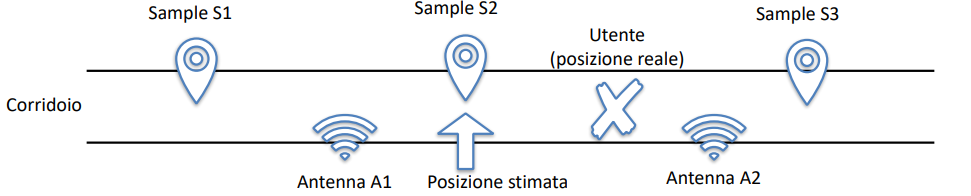
\includegraphics[width = \textwidth]{images/MobiDEV/1. posizionamento indoor/fingerprinting 2.PNG}

Il fingerprint calcolato dell'utente è [$<$A1, 0,3$>$, $<$A2, 0,7$>$].
Si procede con il calcolo delle distanze da fingerprint in radio map:
\begin{itemize}
    \item S1: $|$0,3-0,5$|$ + $|$0,7-0,01$|$ = 0,2 + 0,699 = 0,899
    \item S2: $|$0,3-0,4$|$ + $|$0,7-0,6$|$ = 0,1 + 0,1 = 0,2
    \item S3: $|$0,3-0,1$|$ + $|$0,7-0,8$|$ = 0,2 + 0,1 = 0,3
\end{itemize}
La distanza è minore rispetto ad S2 e quindi assumo che la posizione dell'utente sia quella di S2. 

Se tutto va bene trovo effettivamente il fingerprint vicino alla mia posizione. Se in fase di calibrazione ho collezionato pochi fingerprint l’errore potrebbe essere ampio, ad esempio se in un corridoio ho un fingerprint ogni 10 metri, l’errore potrebbe essere anche di 5 metri. 

Se invece, per via dei dati inesatti, scelgo un fingerprint che non è il più vicino alla mia posizione, l’errore potrebbe essere anche più grande.
\\ Per risolvere questo problema, calcolo la stessa distanza di prima ma al posto di prendere il più vicino, considero i due campioni più vicini e assumo che la posizione dell'utente sia tra quei campioni. 

Prendiamo sempre come esempio il corridoio. \\
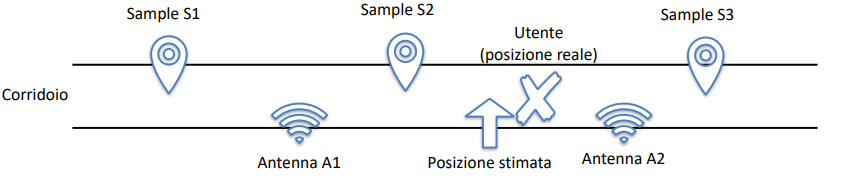
\includegraphics[width=\textwidth]{images/MobiDEV/1. posizionamento indoor/fingerprinting 3.PNG}
Si procede con il calcolo delle distanze da fingerprint in radio map, come nel caso precedente:
\begin{itemize}
    \item S1: $|$0,3-0,5$|$ + $|$0,7-0,01$|$ = 0,2 + 0,699 = 0,899
    \item S2: $|$0,3-0,4$|$ + $|$0,7-0,6$|$ = 0,1 + 0,1 = 0,2
    \item S3: $|$0,3-0,1$|$ + $|$0,7-0,8$|$ = 0,2 + 0,1 = 0,3
\end{itemize}
Successivamente stimo che la posizione dell'utente sia tra S2 ed S3 ad una distanza da S2 di 0,2 / (0,2+0,3) rispetto alla distanza totale tra S2 ed S3.

Abbiamo diversi problemi: la tecnica non è robustissima, abbiamo i dati che sono approssimativi, l'ambiente può cambiare (una porta che si apre o chiude influenza il radiomap), il numero di persone nell'ambiente influenza la radiomap, il tipo di antenna del device, l'umidità.

Bisogna avere quindi un sistema più robusto che riesca a gestire tutti questi fattori, quindi si usano tecniche probabilistiche o basate su machine learning (es: reti neurali).

C'è un altro problema, la fase di setup è molto onerosa. 
Ogni misurazione può durare anche decine di secondi. 
Ci sono vari modi per risolvere il problema:
\begin{itemize}
    \item interpolazione: l'incaricato parte da un certo punto, cammina con velocità regolare, il sistema misura la potenza del segnale e l'incaricato arriva al punto di destinazione. Il sistema sa interpolare i punti, avendo il punto di inizio e quello di fine e la velocità che è costante, l'applicazione calcola i vari fingerprint lungo il percorso
    \item robot: un sistema basato su ruote. In questo modo è più facile misurare lo spostamento. I robot esplorano l'ambiente, sappiamo quanto si spostano, in base a quanto girano le ruote
    \item crowdsourcing: non faccio fare la lettura all'incaricato ma faccio in modo che i dati vengano inseriti dagli utenti finali
\end{itemize}

\subsection{Le tecniche a confronto}

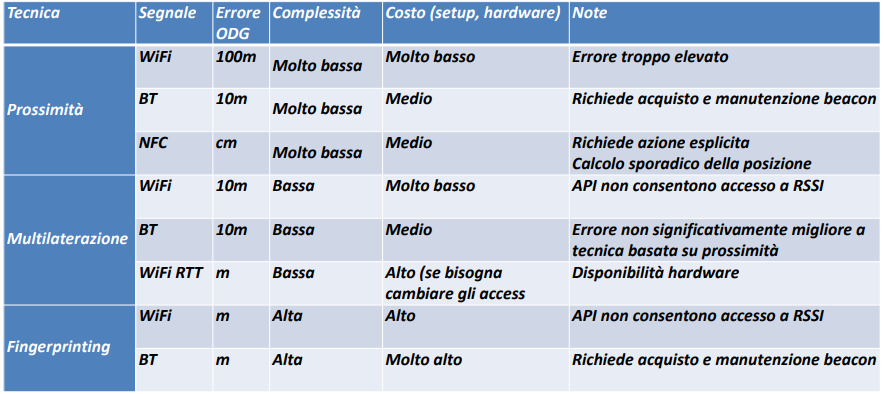
\includegraphics[width = \textwidth]{images/MobiDEV/1. posizionamento indoor/3 tecniche radio.PNG}

\begin{itemize}
    \item prossimità: hanno una minor precisione ma una maggior semplicità, hanno una costo ridotto
    \item multilaterazione: compromesso tra precisione e semplicità ma non aumentano in modo significativo la precisione
    \item fingerprinting: costo alto e complessità alta
\end{itemize}

\section{Sensori inerziali: calcolo dello spostamento}
Ci sono tecniche che permettono di calcolare la posizione come tecniche di dead reckoning utilizzate in diversi ambiti come in quello militare. Viene utilizzato un sommergibile che quando emerge, viene calcolata la posizione con GPS. Durante l'immersione, il segnale sotto una certa profondità non capisce più la posizione, per questo vengono sfruttati gli accelerometri che permettono di misurare l'accelerazione istantanea, dunque otteniamo lo spostamento. 

\textit{Si può usare in dispositivi mobili?}
\\ A bordo del sommergibile ci saranno accelerometri sicuramente più sofisticati rispetto ai telefoni. I sensori inerziali sono soggetti a meno rumore rispetto ad un telefono tenuto in mano mentre si cammina. 

Le tecniche inerziali vanno combinate con altre tecniche perché da sole non calcolano la posizione ma calcolano solo lo spostamento.
Un modo per rendere più robuste le tecniche è di combinare le tecniche inerziali con quelle visive. 

Se non conosco l'orientamento dell'utente, non serve a nulla sapere lo spostamento a meno che non usiamo filtri appositi.

\subsection{Gestione dell'errore}
Il sistema è soggetto a molte forme di errore:
\begin{itemize}
    \item potrebbe sbagliare a contare i passi o la loro lunghezza
    \item potrebbe sbagliare a calcolare la direzione
\end{itemize}
A differenza di tutte le altre tecniche, l’approssimazione nel calcolo della posizione cresce linearmente con il 
tempo. 
\\ Ad esempio ho un fix di posizione e orientamento a t=0s (errore zero). A t=2s mi aspetto un errore di posizione e orientamento contenuto: non posso aver sbagliato di tanto, in così 
poco tempo. A t=4s l’errore è dato dall’errore a t=2 più l’errore accumulato tra t=2 e t=4. Sarà sempre contenuto, ma 
generalmente maggiore dell’errore in t=2. A t=60s ho accumulato l’errore in tutti gli istanti precedenti, dunque generalmente avrò un errore ben più grande rispetto a t=2s.

Questo tipo di errore viene anche chiamato drift.

\subsection{Calcolare un passo}
In teoria è possibile calcolare quando l'utente fa un passo processando i dati di accelerometri e giroscopi. 
In termini pratici però sia iOS che Android rendono disponibile un sensore virtuale che calcola questa informazione (usando i dati di accelerometri e giroscopi), dunque è molto semplice ottenerla.
\\ Il limite di queste tecniche è che contano i passi, ma non si conosce la lunghezza del passo.
\\ Esistono diversi lavori finalizzati a calcolare la lunghezza del passo:
\begin{itemize}
    \item molti assumono che il device mobile sia solidale con il centro di massa dell'utente, come ad esempio lo smartphone legato alla cintura
    \item alcuni considerano il caso in cui il device sia tenuto in mano
    \item altri considerano che una persona faccia passi lunghi sempre uguali, in questo modo se conto i passi e so dove si sposta, posso imparare la lunghezza dei passi stessi da usare in futuro
\end{itemize}

\subsection{Tecniche visuo-inerziali}
Usando tecniche di computer vision è possibile stimare come si sta 
spostando-ruotando la camera.
Le tecniche visuo-inerziali combinano i dati dei sensori inerziali con la stima dello spostamento-rotazione ottenuta attraverso l’analisi del 
flusso video.
\\ Questo permette di ottenere una stima dello spostamento-rotazione 
più robusta rispetto al solo uso dei sensori inerziali.
\\ La tecnica è adottata dalle librerie esistenti di augmented reality.

\section{Tecniche ibride}
Combinano più soluzioni per cercare di avere una soluzione più affidabile.
\\ Un esempio di tecnica ibrida ne è il segnale radio usato in combinazione con la computer vision.
\\ Se ho due stanze identiche in piani diversi, con la tecnica computer vision risulta impossibile identificare la posizione esatta di un utente, per questo viene combinata con il segnale radio. 

Un'altra tecnica è l'utilizzo dei marcatori visivi con il calcolo della posizione. Non puoi chiedere ad un utente di spostarsi inquadrando sempre un marcatore, quindi uso i marcatori visivi. 
\\ Mentre l'utente si sposta uso le tecniche di spostamento, il problema è che dopo un po' la posizione non sarà più calcolata perfettamente, in quanto le tecniche di spostamento accumulino l'errore.
\\ Per azzerare l'errore, l'utente inquadra un marcatore visivo in modo tale che venga fatto anche un fix di posizione. 

\subsection{Tecniche ibride e calibrazione crowsourced}
In questo caso uso più tecniche di posizionamento. 
Quando una tecnica mi fornisce una posizione con buona approssimazione, ad esempio un utente inquadra un marcatore, oppure utente passa vicino ad un beacon, utilizzo questa informazione per calibrare le altre tecniche. Ad esempio tengo traccia della potenza delle antenne WiFi in quella precisa posizione.
Questo procedimento è analogo a quanto avviene in outdoor.

\chapter{Reti e architetture}
\lhead{Reti e architetture - Mobile Computing}
\rhead{Lezione 2 - 6 ottobre}
\begin{center}
    \textbf{--------- Lezione 3 - 6 ottobre 2020 ---------}
\end{center}

\section{Le reti cellulari}
Le reti cellulari permettono ad un dispositivo mobile di trasmettere voce e dati attraverso un'infrastruttura distribuita nel territorio composta da:
\begin{itemize}
    \item Antenne: sono sparse nel territorio ed ognuna di queste ha una copertura limitata. Per permettere ai dispositivi di avere una copertura sufficiente (una copertura geografica), ci sono molte antenne
    \item Varie componenti di elaborazione delle informazioni 
\end{itemize}

Nascono negli anni ’80 e si sono rapidamente evolute. Esempi di tecnologie: GSM, GPRS, EDGE, LTE.
\\ Queste tecnologie sono organizzate in generazioni (es. 1G, 2G, 3G, ecc.) dove ogni generazione stabilisce delle performance di riferimento. 
Le diverse tecnologie condividono una stessa architettura.

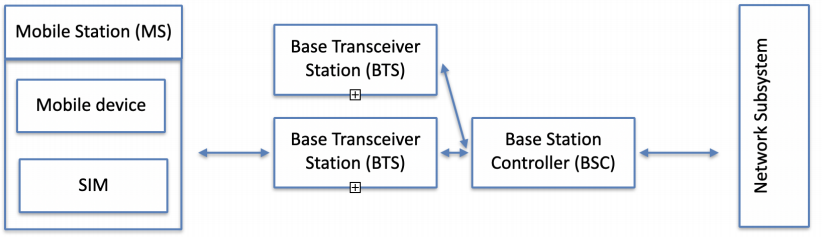
\includegraphics[width=\textwidth]{images/Mobile computing/3. Reti e architetture/architettura.PNG}

La \textit{SIM} è una componente HW che ha la scopo di identificare e autenticare l'utente per l'accesso alla rete. 
Le \textit{Mobile Station (MS)} includono due componenti: la SIM e il device.
La SIM contribuisce a funzioni di sicurezza in quanto contiene chiavi crittografiche utilizzate per realizzare la comunicazione di rete. 
\\ La mobile station comunica via radio con una componente chiamata \textit{Base Transceiver Station (BTS)} che include una o più antenne per la comunicazione e un hw di gestione dell'informazione per gestire il segnale in ingresso e in uscita. Ogni BTS è collegata al \textit{Base Station Controller (BSC)} che coordina varie BTS e a sua volta comunica con l'infrastruttura di rete chiamata \textit{Network Subsystem}. 

La potenza del segnale diminuisce all'aumentare della distanza tra la MS e l’antenna.
La distanza massima di comunicazione dipende dal tipo di tecnologia.
ma in linea di massima entro la quale si può comunicare è anche di diversi chilometri. 
Per erogare il servizio su una scala geografica, sono sparse nel territorio le BTS. 
Ciascuna BTS definisce una cella, cioè una regione geografica dove il segnale di quella BTS è più forte, rispetto al segnale delle BTS circostanti. 
Man mano che ci allontaniamo dall'antenna entriamo in un'altra cella perché il segnale di quest'altra antenna è più forte della precedente. 

Ogni BTS comunica con varie MS tramite onde radio, su intervalli di frequenze che sono specificati dal protocollo utilizzato.
Ogni intervallo è suddiviso in un numero finito di portanti che sono a loro volta suddivise in uplink e downlink (comunicazione verso la BTS).
Ad esempio GSM ha 248 portanti nell'intervallo attorno ai 900MHz.
\\ Ogni portante è suddivisa in canali usando tecniche di FDM (frequency division multiplexing) e TDM (time division multiplexing).
\\ Ogni MS nel momento in cui comunica con la BTS necessita di un canale in uplink e uno in downlink. Il numero massimo di MS che possono comunicare con una stessa BTS è limitato. 
In zone ad alta densità di popolazione è necessario avere celle più piccole, per suddividere la popolazione tra più BTS.
In questo caso una procedura, chiamata session handover, permette il passaggio di controllo di una mobile station ad un'altra e il dispositivo non si accorge di essere passato da un'antenna all'altra. L'IP del telefono rimane invariato. 

\section{Le architetture per dispositivi mobili}
Molto spesso le applicazioni di dispositivi mobili fanno parte di un sistema distribuito e comunicano con un server ed altri dispositivi mobili. 

Ci sono fattori che influenzano molto la progettazione della app:
\begin{itemize}
    \item la connessione potrebbe andare persa. Nei dispositivi mobili è anche normale che l'accesso ad Internet avvenga tramite diversi tipi di connessione che cambiano nel tempo
    \item il tipo di connessione cambia. In alcuni casi grazie al session handover è possibile mantenere la stessa connessione anche quando un dispositivo si sposta all'interno di una rete cellulare, ma la stessa funzionalità non è disponibile quando un dispositivo si sposta tra reti diverse e dunque riceve un nuovo indirizzo IP. Ad esempio un utente è connesso alla rete WiFi di casa, quando esce si connette alla rete cellulare e quando arriva a lavoro si connette ad un'altra rete WiFi che gli assegnerà un nuovo IP
\end{itemize}

\subsection{Connection-oriented vs connection-less}
I due fattori portano a sconsigliare l'utilizzo di protocolli connection-oriented dove si ha una connessione prolungata tra le due entità che comunicano.
Non è consigliabile perché il dispositivo perde la connessione e siccome ho una connessione aperta tra client server, se il client cambia l'indirizzo IP, la connessione va persa.

Nei protocolli connection-less invece non viene mantenuta una connessione prolungata tra due componenti. 
Queste comunicazioni sono più adatte ai dispositivi mobili. 

In un'architettura client-server, il server espone delle API (chiamate) che i client possono sfruttare per portare a termine il loro compito. 

\subsection{Architettura three-tier}
Lo schema architetturale three-tier è comunemente utilizzato per erogare servizi web. 
Il browser fa una richiesta HTTP al web server che legge e scrive i dati su un DB. Una volta che il web server termina la scrittura e la lettura dei dati, esegue lo script lato server, recupera il file necessario ed esegue il codice PHP che può richiedere di interagire con una base di dati. Il web server al browser ritorna la pagina html, il codice javascript che esegue lato client e dei css.
\\ PHP è lo scripting lato server e non viene eseguito lato client, javascript invece è lo scripting lato client e non viene eseguito lato server.

L'architettura per i dispositivi mobili è molto simile.
L'applicazione comunica con un web service tramite HTTP. Il web spesso comunica con un DB che memorizza l'informazione in modo persistente. 
Una delle differenza principali è che l'applicazione client
solitamente riceve dal web service solo i dati richiesti, in quanto il comportamento dell'applicazione, incluse le informazioni su come formattare i dati ricevuti, fanno già parte dell'applicazione stessa. I dati possono essere scambiati in un qualunque formato, incluso il testo semplice. Tuttavia, per dati complessi esistono vari formati, tra cui XML e JSON.

\begin{figure}
    \centering
    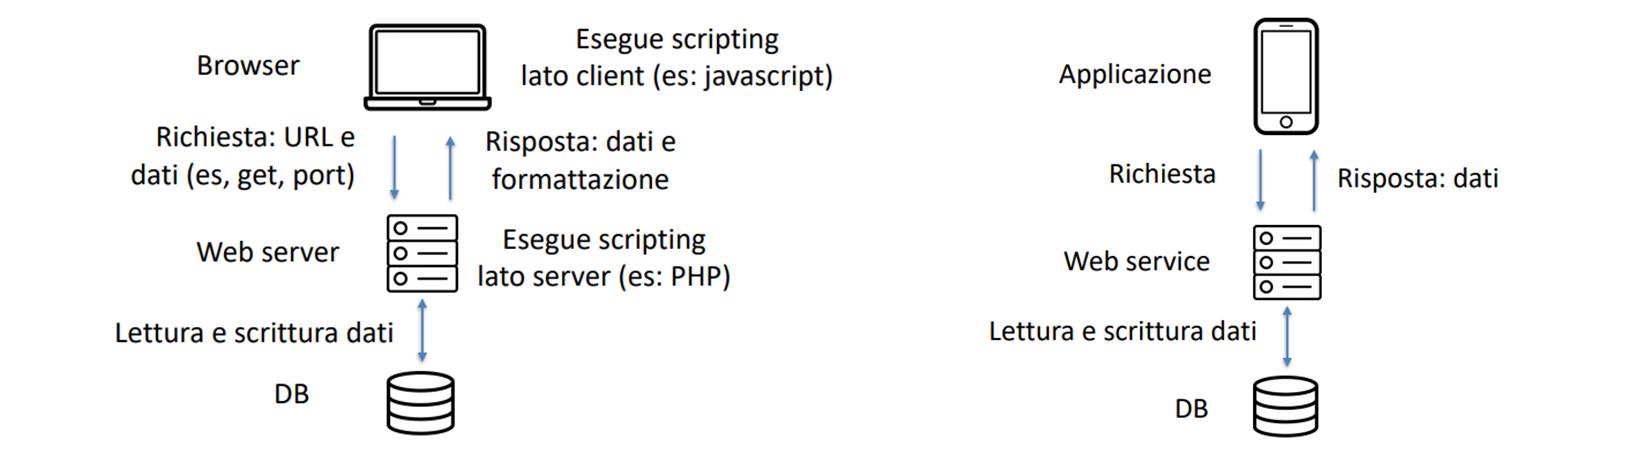
\includegraphics[width=\textwidth]{images/Mobile computing/3. Reti e architetture/architettura tt.png}
    \caption{Schema del modello three-tier applicato al web (sinistra) e alle applicazioni (destra)}
    \label{fig:architettura tt}
\end{figure}

I modelli presentano due componenti diversi:
\begin{itemize}
    \item web server: un server che fornisce informazioni (generalmente HTML+CSS+JS) finalizzate ad essere mostrate (tramite un browser) all'utente 
    \item web service: un server fornisce informazioni finalizzate ad essere ricevute da un’applicazione (anche mobile)
\end{itemize}

Quando facciamo un sistema vero, vogliamo far si che un sistema sia utilizzabile sia su app che su web e vorremmo evitare di scrivere due volte il codice.
Quello che si fa è usare un web server che manda tutti i contenuti al browser e che gli permettono di avere lo stesso comportamento dell'app mobile. 
\\ Invece di avere web service e web server, abbiamo un web service che interagisce con l'applicazione e poi il web server che passa semplicemente al browser la web app. 

\begin{figure}[!ht]
    \centering
    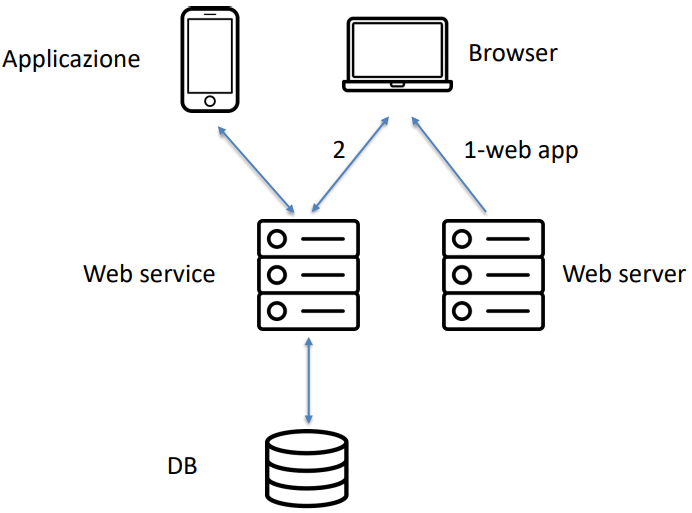
\includegraphics[width=.5\textwidth]{images/Mobile computing/3. Reti e architetture/app_web.PNG}
    \caption{Architettura per supportare contemporaneamente l'accesso da browser e da applicazioni}
    \label{fig:sistemi web_app}
\end{figure}

\subsection{La definizione del protocollo di comunicazione}
Progettare un protocollo di comunicazione non è facile. Vogliamo definire API sul server con le quali i client possono interagire: scambiare i dati con il server e ottimizzare il volume di dati scambiati, tenendo conto dei vincoli dei dispositivi mobili e permettendo una buona esperienza utente. 

Il protocollo è di tipo connection-less. Le chiamate avvengono con connessioni diverse, ma solitamente sono logicamente legate le une alle altre. Bisogna definire in quale ordine avvengono, in quali situazioni, quali dati si devono scambiare, ecc.

\subsubsection{Esempio di comunicazione}
Pensiamo ad un social. Ogni utente ha un profilo (con nome e foto) e uno stato (online o offline). Vogliamo che un utente possa scaricare la lista degli amici. 
\\ Il modo più semplice per implementare questa cosa è richiedere al server l'elenco dei contatti. 
È una soluzione semplice, ma ogni volta che l'utente vuole accedere alla lista, deve riscaricare tutti i contatti (con la foto, il nome e lo stato). 

Un'altra soluzione sarebbe di andare a scaricare in locale gli amici, in modo tale che una seconda volta scarico solamente quelli che precedentemente non avevo ancora scaricato (ad esempio un nuovo amico).
Qui ho un altro problema, perché se un amico aggiorna la foto profilo, io in locale ho quella vecchia. 

La soluzione corretta e ottimizzata è quella di utilizzare un contatore. Per ogni utente il server gestisce un contatore delle foto di profilo caricate (un numero di versione). Quando un utente scarica l’elenco degli amici il server gli manda, per ciascuno, il numero di versione della foto (è un dato di dimensione irrilevante rispetto ad un’immagine). Per ogni amico verifico se ho già salvato in locale la foto giusta e nel caso la mostro, altrimenti chiedo la foto al server e poi la salvo in locale per la prossima volta.

\begin{figure}[!ht]
\begin{center}
    \subfloat[Aggiornamento delle foto]{\fbox{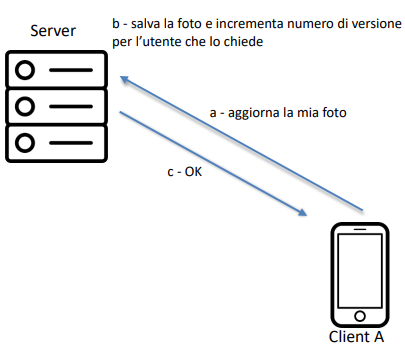
\includegraphics[width=.4\textwidth]{images/Mobile computing/3. Reti e architetture/1.PNG}}}
    \qquad \subfloat[Scarico lista amici]{\fbox{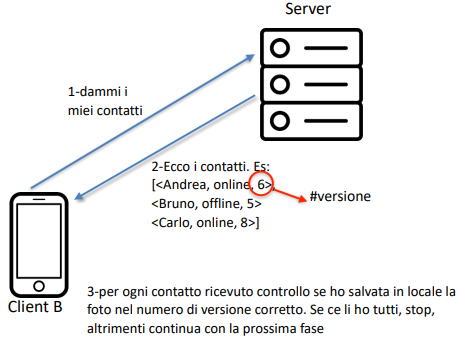
\includegraphics[width=.45\textwidth]{images/Mobile computing/3. Reti e architetture/2.PNG}}}
    
    \subfloat[Scarico foto aggiornate]{\fbox{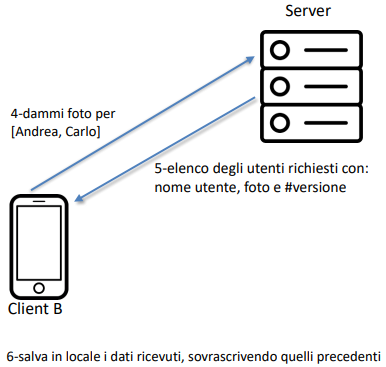
\includegraphics[width=.4\textwidth]{images/Mobile computing/3. Reti e architetture/3.PNG}}}   
\end{center}
\caption{Trasmissione delle immagini profilo in un social network}
\label{fig:immagini social}
\end{figure}
\newpage

\section{La codifica dell'informazione}
In una richiesta HTTP è possibile trasmettere informazioni in testo semplice. 

Prendiamo ad esempio un servizio che prende una parola in input e risponde con un sinonimo.
L'output è sempre una stringa e se non viene trovata nessuna corrispondenza, ritorna la stringa vuota.

Prendiamo ad esempio, invece, un servizio che data una parola in input risponde con una lista sinonimi. 
In questo caso potremmo ad esempio usare una codifica di parole separate da virgole. 

Diventa peggiore se data una parola in input, risponde con una lista di sinonimi e una di contrari.
Dobbiamo rappresentare due liste di parole e potemmo inventarci un modo per separare le due liste, per esempio usare il punto e virgola per separare.

Esistono degli strumenti che ci permettono di codificare l'informazione come ad esempio XML e JSON.

XML è un linguaggio di markup che permette di definire formati dei dati che sono “human and machine readable”. 

Un documento XML è ben formattato se rispetta alcune regole (ad esempio se tutti i tag sono aperti e poi chiusi). 
XML presenta alcuni limiti:
\begin{itemize}
    \item tende ad essere verboso 
    \item non facilmente leggibile da umani
    \item gli schemi XML sono abbastanza difficili da definire e spesso vengono ignorati
\end{itemize}

Un esempio di risposta XML per il servizio dictionary:
\begin{XML}
    <dictionary entry="nice">
        <synonyms>
            <word>pleasant</word>
            <word>agreeable</word>
            <word>enjoyable</word>
        </synonyms>
        <antonyms>
            <word>ugly</word>
            <word>unpleasant</word>
        </antonyms>
    </dictionary>
\end{XML}

JSON concettualmente svolge lo stesso lavoro di XML, cerca di ridurre la verbosità e di migliorare la lettura. 
\\ Un esempio di risposta JSON per il servizio dictionary:
\begin{JSON}
    {
        "entry":"nice",
        "synonyms ":[" pleasant","agreeable","enjoyable"],
        "antonyms ":[" ugly","unpleasant"]
    }
\end{JSON}    

XML definisce delle entità, JSON definisce degli oggetti. 
Sono due rappresentazioni diverse, ma concettualmente sono analoghi, infatti rappresentano i dati di un elemento che vogliamo descrivere.

Un'entità in XML o un oggetto JSON mi definisce uno stato nel mondo reale ma non il comportamento, nei linguaggi di programmazione invece un oggetto definisce sia lo stato che il comportamento ad esso associato. 
Questa distinzione è molto importante in quanto esiste una forte correlazione tra le strutture dati dei programmi e la codifica in XML o JSON. 

\subsection{Serializzazione e deserializzazione}
In memoria principale lavoriamo con oggetti dei linguaggi di programmazione ma questi oggetti non possono transitare in rete. Quello che ci serve è andare a convertirli nella propria rappresentazione XML o JSON. Questa operazione si chiama \textit{serializzazione} (o \textit{marshalling}). Il risultato è una stringa (internamente codificata in XML o JSON). L'entità che riceve la comunicazione di rete può leggere questa stringa e
riconvertirla in struttura dati tramite un’operazione che si chiama \textit{deserializzazione} o \textit{unmarshalling}.
Uno dei vantaggi nell'uso di XML o JSON è che le operazioni di serializzazione e deserializzazione sono supportate, in quasi tutti i linguaggi di programmazione, da apposite librerie.
Un esempio di queste librerie è GSON. 
\\ GSON è lo strumento di conversione, JSON è il formato di rappresentazione.

\subsection{Codifica di dati binari}
Sia in XML che in JSON vengono rappresentati i dati singoli nella loro codifica testuale. Non c'è nessun problema per stringhe, interi, float, boolean, ecc, ma si pone un problema per i dati binari ad esempio le immagini.
Il modo più comune è la codifica Base64 che permette di rimappare la codifica binaria dell'informazione in alcune informazioni testuali.
\\ Definisco una conversione tra 64 simboli (caratteri ASCII) e un valore numerico: A=1, B=2, ecc.
Scelgo dei caratteri ASCII che non mi introducano confusione nelle rappresentazioni XML o JSON (es: non uso "$<$", né ",").
Un simbolo rappresenta dunque 6 bit ($2^6$ = 64).
Dunque per rappresentare 3 byte in binario mi servono 4 simboli (3*8 = 4*6).
Per convertire da binario a Base64 suddivido l’input in gruppi di 3 byte, codifico ciascun gruppo con 4 simboli Base64.
Si usa la Base64 perché è una codifica testuale che usa meno caratteri per rappresentare e perché permette di non utilizzare caratteri strani. 

\subsection{Protocol Buffer}
Protocol Buffer è il protocollo definito da Google per serializzare le informazioni. Risolve lo stesso problema di XML e JSON definendo non solo il formato di scambio, ma anche gli strumenti SW di (de)serializzazione.
\\ Protocol Buffer è un protocollo:
\begin{itemize}
    \item multi-piattaforma, multi-linguaggio 
    \item ottimizzato in termini di dimensione del messaggio da scambiare 
    \item che risolve diversi problemi tipici ad esempio la gestione della versione dei protocolli 
\end{itemize}
\vspace{2em}
\rhead{Lezione 2 - 7 ottobre}
\begin{center}
    \textbf{--------- Lezione 4 - 7 ottobre 2020 ---------}
\end{center}

\section{Le notifiche push}
Nei protocolli di comunicazione abbiamo visto che è preferibile fare in modo che sia un’applicazione per dispositivi mobili a contattare un server e non viceversa. 
Ci sono però dei casi in cui non è possibile, se c'è un evento che si genera sul server, è il server stesso che deve contattare il client. 
\\ Ho diverse soluzioni:
\begin{itemize}
    \item mantenere una comunicazione aperta rispetto al server, ad esempio via TCP. 
    \\ Questa soluzione non va bene, è meglio evitare approcci connection-oriented
    \item il client rimane in attesa di connessione, esempio con un server socket. 
    Anche questa soluzione non va bene, il client non dovrebbe rimanere in ascolto di connessioni da parte del server
    \item il client fa polling: "hai qualche messaggio per me?"
    La soluzione non va bene in quanto sia costosa, dato che il client continua ad interrogare il server senza ricevere, nella maggior parte dei casi, nessun aggiornamento
    \item BOSH: permette al client di fare una richiesta HTTP al server e risponde subito se ha qualcosa. Se non ha niente, tiene la richiesta HTTP in attesa fino a quando non ha nulla da comunicare. 
    Può succedere che il client si disconnetta o che il client cambi IP. La richiesta fallisce e il client ne fa una nuova.
    Anche qui la soluzione richiede che il client sia sempre in esecuzione
\end{itemize}

C'è una soluzione ottimale, rispetto a quelle precedenti, che è quella delle \textit{notifiche push}. Si tiene un solo servizio attivo a livello di SO per ricevere comunicazioni asincrone. 
Questa soluzione fa in modo che sia il SO a rimanere in attesa di comunicazioni da un server esterno, dunque con una sola connessione, offrendo poi il servizio alle altre applicazioni. 

\subsection{Componenti delle notifiche}
Ci sono diverse componenti coinvolte:
\begin{itemize}
    \item l'\textbf{utente} che usa il dispositivo mobile
    \item \textbf{SO} del device
    \item \textbf{app} che deve ricevere la notifica
    \item \textbf{push server}, un servizio esterno che comunica con il SO (sviluppato da Apple e Google). Offre il servizio di push notification
    \item \textbf{app server}, un server che vuole inviare comunicazioni asincrone all'app
\end{itemize}

\subsection{Il protocollo}
Il protocollo alla base delle notifiche push è suddiviso in due fasi: setup e invio.

È necessario introdurre un elemento fondamentale del protocollo, il \textit{device token} che identifica la coppia data dal dispositivo e dell'applicazione ($<applicazione, device>$) che vuole ricevere le notifiche push. Il device token è creato dal push server usando tecniche crittografiche che garantiscono che il device token non possa essere creato da altri e che, una volta creato, non possa essere modificato.

\subsubsection{La fase di setup}
La fase di setup viene iniziata dall'app. Voglio permettere all'app server di mandare delle notifiche. 
Lo scopo è quindi quello di fare arrivare il device token all'app server. 
 
Il procedimento è il seguente.

\begin{figure}[!ht]
    \centering
    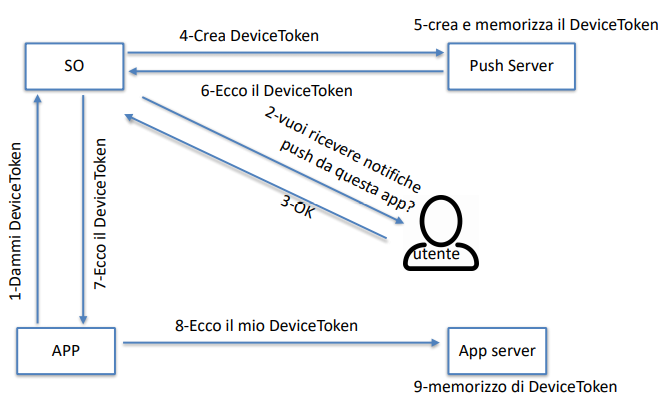
\includegraphics[width=.65\textwidth]{images/Mobile computing/3. Reti e architetture/setup.PNG}
\end{figure}

L'app fa una chiamata di API al SO che chiede all'utente se vuole autorizzare l'applicazione ad inviare le notifiche push. Se l'utente non autorizza, il procedimento finisce, se invece autorizza il SO chiede al Push Server di creare il DeviceToken. 
Il Push Server lo crea, lo memorizza e lo manda al SO. 
Il SO risponde all'app dando il DeviceToken. 

La richiesta "1. Dammi DeviceToken" è una chiamata bloccante oppure asincrona. 
L'app riceve il DeviceToken e lo comunica all'App server. 


\subsubsection{Fase di invio}
La fase di invio delle notifiche, invece, viene eseguita ogni volta che l’app server vuole mandare una comunicazione asincrona all’applicazione. 

Lo scopo è quindi di fare arrivare, tramite l'app server, all'app un messaggio con un piccolo payload. Il payload è il testo da mostrare ed eventuali altre informazioni come ad esempio "Hai 5 nuovi messaggi".

Il procedimento è il seguente. 
\begin{figure}[!ht]
    \centering
    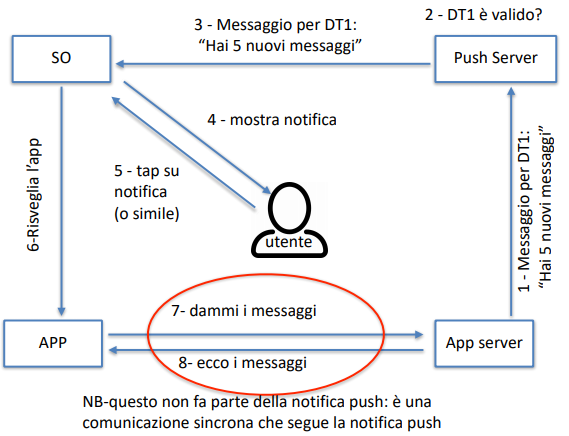
\includegraphics[width=.65\textwidth]{images/Mobile computing/3. Reti e architetture/invio.PNG}
\end{figure}

L'app server contatta il push server dicendo che ha un nuovo messaggio e allega due informazioni: il device token memorizzato in fase di setup e i payload. Il messaggio tra app server e push server è un messaggio tra due computer in rete. 
Il push server verifica che il device token sia valido e se è valido contatta il SO in modo asincrono, per esempio tramite l'implementazione di un protocollo simile a BOSH. Se il push server non riesce a contattare il SO, memorizza l'informazione della richiesta (ad esempio quando il telefono è spento o non ha connessione). 
Il SO mostra la notifica all'utente con anche il testo contenuto nel payload. L'utente fa il tap sulla notifica e il SO risveglia l'app.

\subsection{Attacchi}
Il protocollo alla base delle notifiche push fornisce garanzie di sicurezza più elevate rispetto ad altri servizi (ad esempio l'email).
Il push server può agire attivamente per prevenire gli attacchi. Alcuni esempi di attacchi che si possono prevenire sono:
\begin{itemize}
    \item \textbf{spamming}: un'app server non può inviare notifiche push ad un client che non lo ha autorizzato, perché non dispone del device token
    \item \textbf{impersonificazione}: un'app server non può far finta di essere un altro app server (es: telegram non può mandare una notifica push facendo finta di essere whatsapp). Questo aiuta a prevenire gli attacchi di tipo phishing (truffe) 
    \item \textbf{messaggi indesiderati}: se un app server inizia a mandare troppi messaggi o messaggi indesiderati all’utente, l’utente ha la possibilità di revocare il device token
    \item \textbf{flooding}: il push server può bloccare le richieste, se ad esempio un app server (anche autorizzato) prova ad inviarne un numero eccessivo allo stesso device
\end{itemize}

\subsection{Notifiche push e locali}
I SO rendono disponibili due tipi di notifiche: push e locali.
È facile fare confusione perché sono presentate in modo simile all'utente, ma sono completamente differenti da un punto di vista architetturale.
Le notifiche locali vengono generate dall'app stessa mediante delle chiamate al SO, di solito per dare informazioni all'utente quando l'app è in background (es: app di navigazione), oppure per mandare reminder all'utente ad orari prestabiliti.


\chapter{Calcolo e uso della posizione}
\lhead{Calcolo e uso della posizione - Mobile Computing}
\section[Introduzione all'uso dell'informazione di posizione]{Introduzione all'uso dell'informazione di \\posizione}
La posizione ci indica dove si trova un dispositivo in un ambiente di riferimento che può essere nel mondo, in un edificio, ecc. 
\\ Possiamo avere 2 dimensioni, dove la posizione è considerata rispetto ad un piano, oppure 3 dimensioni, dove la posizione è considerata rispetto ad un piano ed un'altezza.
Possiamo rappresentare la posizione attraverso la:
\begin{itemize}
    \item rappresentazione geografica: la posizione nel mondo 
    \item rappresentazione in coordinate locali: la posizione ad es. su una mappa 
    \item rappresentazione semantica: es. indirizzo
\end{itemize}

Nella rappresentazione geografica ci sono due sistemi di riferimento: 
\begin{itemize}
    \item latitudine: viene preso come punto di riferimento l'equatore 
    \item longitudine: viene preso come riferimento il meridiano di Greenwich 
\end{itemize}

L’informazione di posizione non riporta il tempo, ma l'informazione temporale è fondamentale da associare alla posizione in molti contesti, ad esempio se vogliamo descrivere una traiettoria, cioè una lista di elementi $<$timestamp, position$>$. 

Il calcolo della posizione (e del tempo) non è esatto. 
In termini matematici potremmo definire una funzione, di distribuzione di probabilità, che associa ad ogni punto dello spazio la probabilità che il device si trovi lì. 
In termini pratici, si modella un'area dove probabilmente si trova il device. 
Questa approssimazione però non ci dice dove si trova il device all'interno dell'area. 

\subsection{Accuratezza e precisione}
Una delle caratteristiche più rilevante di un sistema di calcolo della posizione è quanto la posizione calcolata differisce da quella reale. 
\\ Supponiamo che l’utente sia fermo e che siano date varie misurazioni della sua posizione.
Con \textit{precisione} si intende quanto le misurazioni sono vicine l'una all'altra.
Con \textit{accuratezza} si intende quanto le misurazioni siano vicine alla posizione vera.

L'errore di posizionamento viene calcolato in questo modo: indico che la posizione calcola ha un x\% di probabilità di probabilità di essere più vicina di y metri alla posizione corretta. 

Il livello di precisione non sempre è lo stesso, dipende dal tipo di applicazione e dal tipo di utente. 
Possono avere una precisione a livello di: 
\begin{itemize}
    \item regione (fino a 200km): meteo, news, etc… 
    \item area metropolitana (fino a 20km): local news, traffico, ecc.
    \item quartiere-città (fino a 2km): gestione flotte 
    \item isolato (50-100m): gestione emergenze, pubblicità geo-referenziata, informazioni sui POI (Point Of Interest) 
    \item dintorni dell’utente (5-50m): navigazione outdoor, taxi, car sharing 
    \item prossimità dell’utente (1-5m): navigazione indoor
\end{itemize}

Oltre alla posizione siamo anche interessati a conoscere 
l'orientamento, che può assumere diversi significati:
\begin{itemize}
    \item come è orientato, sui tre assi, il device 
    \item in quale direzione (2D) è direzionato l’utente (heading). Heading lo posso misurare con i sistemi inerziali
    \item in quale direzione (2D) si sta muovendo l’utente (course)
\end{itemize}
Ad esempio quando ci spostiamo con il navigatore e non sa dove stiamo guardando, finché non iniziamo a muoverci non riesce a darci le indicazioni giuste. 

Possiamo capire l'orientamento attraverso:
\begin{itemize}
    \item heading: uso i sensori inerziali per capire dove sta puntando il device
    \item course: vedo in quale direzione si sta spostando l'utente. Posso calcolarlo solo quando ho una traccia di spostamento dell'utente 
\end{itemize}

\subsection{Calcolo della posizione con trilaterazione}
La trilaterazione assume che io debba calcolare la posizione di un oggetto sapendo la distanza da altri oggetti e conoscendo la loro posizione. 
Ci sono diverse varianti: 
\begin{itemize}
    \item numero degli oggetti dai quali conosco la distanza
    \item in che termini conosco la distanza tra X e $O_i$?
    \begin{itemize}
        \item \textbf{distanza esatta}: se conosco la distanza esatta di X da 3 oggetti, posso sapere qual è la posizione di X. 
        \begin{center}
            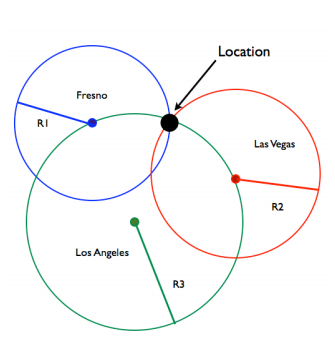
\includegraphics[width=.25\textwidth]{images/Mobile computing/4. Posizione/distanza esatta.PNG}
        \end{center}
        
        \item \textbf{upper bound} della distanza: "la distanza è al più...".
        Molte tecniche forniscono una distanza massima del device da una posizione nota.
        Se ho un solo oggetto so che la posizione sarà all'interno della circonferenza. Se ho due o più oggetti, la X starà nell'intersezione.
        \\ 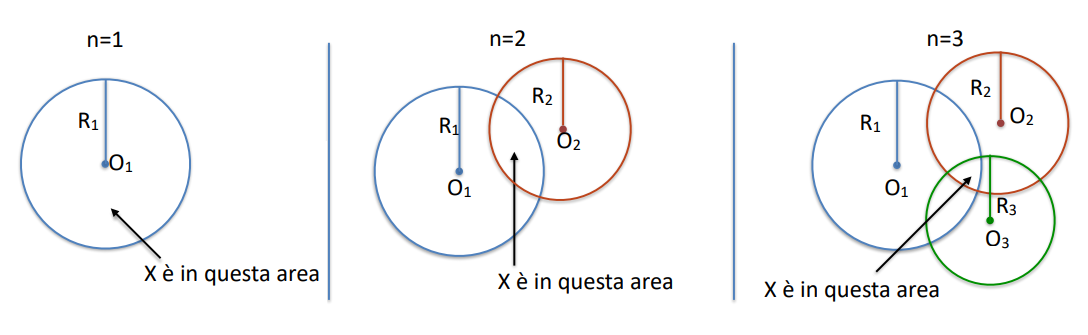
\includegraphics[width=.9\textwidth]{images/Mobile computing/4. Posizione/upper bound.PNG}
        \item \textbf{range di distanza}: "la distanza è compresa tra ...". \\
        \begin{minipage}{.4\textwidth}
           Possiamo definire il problema in modo più generale considerando che per ogni oggetto $O_i$ conosco una distanza minima e massima rispetto ad x
        \end{minipage} 
        \hfill
        \begin{minipage}{.6\textwidth}
            \begin{center}
                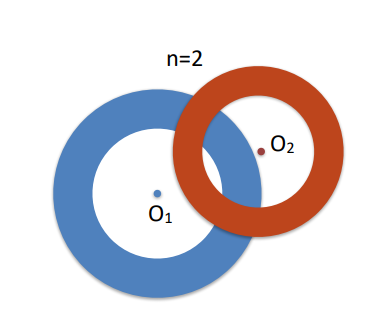
\includegraphics[width=.45\textwidth]{images/Mobile computing/4. Posizione/range di distanza.PNG}
            \end{center}
        \end{minipage}
    \end{itemize}
\end{itemize}

In tutti i casi abbiamo una stima della distanza, ma la stima può essere errata. 
Il sistema di calcolo della posizione deve essere in grado di gestire anche questi casi, ad esempio provando ad identificare la stima errata sulla base delle altre. 
\begin{center}
    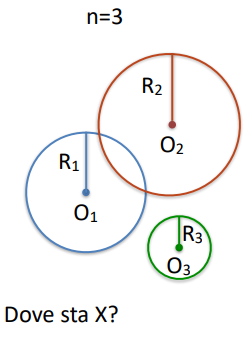
\includegraphics[width=.3\textwidth]{images/Mobile computing/4. Posizione/stima errata.PNG}
\end{center}
In questo esempio posso stimare che la posizione di X sia nell'intersezione tra R1 ed R2 ma nel punto più basso, perché devo anche considerare R3. 

\section{Calcolo della posizione outdoor}
La posizione outdoor si calcola con 3 soluzioni: 
\begin{itemize}
    \item Global Navigation Satellite System (GNSS) 
    \item Rete Cellulare 
    \item WiFi Network based
\end{itemize}
Queste tecniche da sole non funzionano, devono essere combinate con altre tecniche ibride.

\subsection{Global Navigation Satellite System (GNSS) }
Ci sono una serie di satelliti che viene messa in orbita e in ogni istante possiamo sapere la loro posizione.
Hanno a bordo un orologio atomico che gli permette di sapere l'ora in modo preciso.
Mentre i satelliti ruotano, inviano il proprio id insieme all'informazione temporale. 

Il dispositivo mobile riceve l'informazione e riesce a calcolare la distanza da uno o più satelliti. Sfruttando il tempo di propagazione del segnale posso conoscere la distanza dal satellite (la cui posizione può essere calcolata), quindi si usa una tecnica simile alla trilaterazione per calcolare la posizione.

Abbiamo un problema. Il device non ha un orologio atomico, quindi deve essere sincronizzato e richiede di ricevere il segnale da almeno 4 satelliti. Posso calcolare così la mia posizione nello spazio e la mia posizione precisa. 
Possiamo avere anche problemi legati a:
\begin{itemize}
    \item interferenze: in particolare atmosfera (condizioni meteo) e edifici 
    \item posizione dei satelliti potrebbe non essere esattamente quella prevista
\end{itemize}

Ci sono diversi sistemi in uso: 
\begin{itemize}
    \item GPS (USA): è in grado di fornire una posizione maggiore ma per motivi di sicurezza, la precisione sotto ai 3 metri viene usata in ambiti militari
    \item GLONASS (Russia)
    \item Galileo (Europa): fornisce una posizione sotto al metro
\end{itemize}

Ci sono due modi per diminuire i problemi del segnale satellitare:
\begin{itemize}
    \item Differential GPS (D-GPS): è un sistema che permette di correggere (almeno in parte) l'errore dovuto alle interferenze dell'atmosfera e ad una non precisa posizione dei satelliti rispetto a quanto previsto. Consiste nell'avere stazioni terrestri collocate in posizioni note che misurano la potenza del segnale dei satelliti. Un ricevitore in posizione fissa a terra calcola la distanza tra il segnale atteso e quello che effettivamente riceve. Il ricevitore poi comunica questa informazione ai dispositivi mobili che dunque possono compensare l'errore
    \item Assisted GPS (A-GPS): il calcolo iniziale della posizione può essere molto lungo (anche qualche minuto) perché il device deve capire quali satelliti sono in vista. A-GPS risolve questo problema:
    \begin{itemize}
        \item ogni antenna della rete cellulare mantiene un elenco dei satelliti in vista 
        \item quando il device deve usare GPS, richiede, tramite un apposito servizio, quali sono i satelliti in vista all'antenna più vicina. Saranno gli stessi in vista al device (l’antenna non può essere troppo lontana) 
    \end{itemize}
    Questo riduce notevolmente il tempo di calcolo della posizione che in genere è di pochi secondi
\end{itemize}

\subsection{Rete cellulare}
Un altro modo per calcolare la posizione è attraverso la rete cellulare.
Ogni device è connesso ad un'antenna di cui sono note la posizione e l'area della relativa cella. 
Il problema è che l'approssimazione è molto alta e dipende dalla dimensione della cella. 
Una prima soluzione è il protocollo GSM, che prevede l'uso di una tecnica per stimare la distanza tra il device e l'antenna.
Lo scopo all'interno di GSM è quello di evitare collisioni, c'è quindi una tecnica che permette di stimare la distanza tra il device e l'antenna. 

Oltre al protocollo GSM, possiamo sviluppare tecniche per stimare la distanza tra un device mobile e un'antenna dove usiamo il ritardo id propagazione del segnale per stimare la distanza tra un device mobile e un'antenna di rete cellulare. La precisione è nell'ordine di 50-125 metri. 


\subsection{WiFi positioning}
Ci serve conoscere la distanza tra il device e gli Access Point e la posizione di questi. 

Il protocollo 802.11 (protocollo di base alle reti WiFi) prevede che gli access point comunichino il proprio ID, anche ai device che non sono connessi/autenticati a quella rete.
Possiamo sapere quali sono i device che sono nelle vicinanze e la loro relativa potenza del segnale. Minore è la potenza del segnale, significa che sono lontano, maggiore è la potenza del segnale e più sono vicino.

\subsubsection{Problemi}
La potenza del segnale è approssimativamente proporzionale alla distanza perché ci potrebbero essere delle interferenze, infatti se un device e un AP sono vicini, ma c'è qualcosa che crea interferenza, la potenza del segnale sarà bassa.

Un altro problema è che non sappiamo dove sono posizionati gli AP, per questo usiamo un approccio basato su crowdsourcing, un modo di raccogliere i dati dagli utenti che usano il servizio. 
Il crowdsourcing può richiedere o meno un’azione esplicita da parte degli utenti.
Quando l'utente ha il GPS attivo, calcola la propria posizione con una buona precisione e comunica ad un location service (server) la propria posizione e gli access point nelle vicinanze. 
Il location service riceve le informazioni da più utenti e stima la posizione degli access point. 
Quando un utente non ha il GPS attivo: 
\begin{itemize}
    \item invia al location service l'elenco degli AP nelle vicinanze (e la potenza del segnale) 
    \item il location service calcola la posizione dell'utente e gliela comunica
\end{itemize}

Ogni volta che il device vuole calcolare la posizione, guarda quello che ha e lo comunica al location service che risponde con una posizione. 
Questa è una tecnica ibrida perché è basata su due tecnologie, GPS e WiFi.

\textit{Chi calcola la posizione usando il sistema satellitare? Device o server?}
\\ Il device ha l'antenna e può calcolarlo in autonomia. 

Per il calcolo della posizione WiFi non ho in locale la conoscenza delle posizioni degli AP e quindi ho la necessità di comunicare con un location service. 


\rhead{Lezione 2 - 9 ottobre}
\begin{center}
    \textbf{--------- Lezione 5 - 9 ottobre 2020 ---------}
\end{center}

\section{Gestione dei dati di posizione}
Quando il device mobile ha calcolato la posizione, la può usare localmente oppure la può inviare ad un server.

In entrambi i casi si possono adottare tecniche per gestire il dato di posizione. 
Le più comuni sono:
\begin{itemize}
    \item Geocoding e reverse-geocoding: entrambi vengono svolti dal server, geocoding converte l'indirizzo geografico in coordinate spaziali, reverse geocoding è l'operazione inversa
    \item Geofencing: viene svolta in locale dal device, si definisce un'area e il device tiene monitorata la posizione dell'utente quando si entra e si esce dall'area (ad esempio attraverso una notifica)
    \item calcolo delle distanze: esiste una formula che calcola la distanza dalla terra (calcolo in linea d'aria)
    \item calcolo delle distanze su rete stradale: non abbiamo un calcolo in linea d'aria ma si modella la rete stradale come un grafo dove:
    \begin{itemize}
        \item i nodi sono le intersezioni
        \item gli archi sono i segmenti di strada
    \end{itemize}
    Ogni arco è etichettato con la distanza geografica tra i due nodi oppure con il tempo necessario per andare da un nodo all'altro calcolato come:
    \begin{itemize}
        \item tempo: distanza / limite di velocità (non molto affidabile, dipende dal traffico e altri fattori) 
        \item tempo di percorrenza medio di altri utenti
    \end{itemize}
\end{itemize}

Spesso i dati vengono memorizzati lato server dove è necessario definire delle tecniche di trattamento apposite.
\\ Ad esempio molti DBMS utilizzano dati spazio temporali ed offrono delle estensioni a DB classici per gestirli. 

Ci sono tre query comunemente adottate nei servizi e nel DBMS con 
estensioni spaziali:
\begin{itemize}
    \item Range query: si dà in input una zona geografica (che può essere un rettangolo oppure un cerchio) e la query ritorna tutti i punti che appartengono a quella zona indicata. Es: dammi tutte le automobili che sono nel posteggio
    \item Nearest Neighbors (NN): ho un insieme di punti e do in input uno di questi punti. La NN mi ritorna l'oggetto più vicino ad un punto o ad un altro oggetto. Es: dammi le tre stazioni di servizio più vicine a me
    \item Reverse-NN: dato un insieme di punti P e un punto q di P,  ritorna tutti i punti di P che hanno q come punto più vicino. Es: dammi tutti gli utenti che hanno me come loro utente più vicino o dammi tutte le case che hanno quel supermercato come il più vicino
\end{itemize}

I DB implementano delle strutture dati chiamati indici che permettono di rendere le operazioni più veloci. 
\\ Per esempio una range query su un’area “piccola”, rispetto alla distribuzione dei punti, ha una complessità logaritmica nel numero dei punti.





\chapter{Analisi}
\lhead{Analisi - Mobile Computing}
\section{L'analisi delle applicazioni per dispositivi mobili}
Rispetto ad un'analisi del software nei dispositivi tradizionali, nei dispositivi mobili l'utente agisce in un contesto diverso.

Le applicazioni si usano per due motivi:
\begin{itemize}
    \item per risolvere i problemi: l’utente spesso usa le app per risolvere un problema della vita quotidiana, come ad esempio chiamare qualcuno. 
    \item sono pronti all'uso, sono quasi sempre accesi
\end{itemize}

Rispetto ai dispositivi tradizionali, le sessioni d’uso sono mediamente molto brevi, infatti gli utenti vogliono risolvere il loro problema il più velocemente possibile.

L'esperienza dell'utente è un aspetto importante nell'analisi dell'applicazione ed è necessario pensare a come l'utente interagisce con essa. Per questo bisogna eliminare, o minimizzare:
\begin{itemize}
    \item tempi di apprendimento
    \item tempi di set/up e registrazione al servizio
    \item tempi di utilizzo
\end{itemize}

WhatsApp è un esempio tra le prime applicazioni di messaggistica che ha avuto la meglio sulle app concorrenti perché non richiede la registrazione e perché aggiunge automaticamente i contatti tra quelli già presenti in rubrica. 

Uno dei primi giochi che ha basato il suo successo su sessioni di gioco brevissime è Angry Birds, dove una partita può durare alcuni secondi e le istruzioni fornite al primo livello sono presentate in un video di meno di 3 secondi.

\section{Progettazione della user experience}
La user experience (UX) è l'interazione che c'è tra uomo macchina, ciò che una persona prova quando usa un prodotto. 
Include vari aspetti: esperienza nell’uso, utilità, semplicità d’uso
La UX estende:
\begin{itemize}
    \item il concetto di usabilità: è semplice da usare?
    \item il concetto di user interface (UI), una componente della UX
\end{itemize}

Un'app deve: 
\begin{itemize}
    \item avere le funzionalità richieste
    \item funzionare come previsto
    \item essere usabile dall'utente
    \item dare soddisfazione all'utente
\end{itemize}
Tutte queste componenti contribuiscono a formare la UX.

La cosa più importante è che dobbiamo pensare all'utente. 
L'utente vuole risolvere il problema, non vuole sapere la struttura dati o le chiamate al server effettuate a livello programmativo. 
Un aspetto a cui bisogna prestare attenzione è il fatto che le icone e il testo debbano essere scelti con attenzione.

Correggere un errore in fase di analisi costa poco, invece correggerlo in fase di testing, il costo è più elevato in quanto si debba tornare nella fase di analisi e rifare tutte le fasi successive (analisi, implementazione ecc.).

\subsection{Content Prioritization}
All’utente bisogna presentare i contenuti e le funzionalità più importanti. 
L’utente deve poter accedere a contenuti e funzionalità aggiuntive in un secondo momento, ad esempio attraverso un menù. 

Dobbiamo conoscere gli utenti, è necessario sapere a cosa sono interessati. Deve essere effettuata un'analisi iniziale con interviste, questionari, ecc. dove vengono coinvolti gli attori e gli altri stakeholder.
Dobbiamo capire: 
\begin{itemize}
    \item il prodotto serve veramente? Quanto valore ha? Come sarà utilizzato? 
    \item quali funzionalità sono più importanti? 
    \item quali problemi possono emergere? 
\end{itemize}

Dobbiamo ad esempio realizzare un'applicazione per la didattica per bambini. In una fase di analisi parlo con i bambini, gli insegnanti, i genitori, ecc. Poi devo pormi delle domande: useranno l’app in classe o a casa? Da soli o con un adulto? 

Dopo che l’app è stata pubblicata posso raccogliere dati di utilizzo come ad esempio quanto spesso l’app viene usata, quali schermate sono mostrate, quali funzionalità sono usate, ecc.
Esistono vari strumenti, ad esempio Google analytics for mobile, che permettono di svolgere un’analisi data driven che influenza le successive attività di sviluppo.

Ci sono diversi fattori da rispettare: 
\begin{itemize}
    \item la semplicità dell'interfaccia grafica: le interfacce grafiche devono essere il più semplici possibili. Negli schermi dei dispositivi mobili lo spazio dedicato ad elementi grafici non indispensabili toglie spazio a quelli indispensabili. 
    Un esempio di interfaccia grafica confusionaria era quella di Virgilio, quella di Google invece è minimale.
    \item integrità estetica: l'aspetto estetico dell'applicazione deve riflettere la natura dell'applicazione stessa. Un'applicazione per la produttività deve avere un aspetto serio, semplice, lineare e non frivolo, mentre un'applicazione ludica deve avere un maggiore spazio alla grafica ricercata, divertente e appassionante. 
    \item consistenza: l'app dovrebbe funzionare e ricordare altre app che l'utente ha già usato. 
    Se abbiamo delle funzionalità nuove, dobbiamo spiegarle all'utente. 
    \item affordance: caratteristica di un oggetto o di un ambiente di "suggerire" a un individuo la possibilità di compiere un'azione. Attraverso il proprio aspetto l'interfaccia deve invitare l'utente a interagire intuitivamente con essa, sfruttando l'esperienza pregressa (accumulata nel mondo reale o nell'uso di altre app), ad esempio "scroll to refresh"
    \item metafore: i riferimenti al mondo reale aiutano a capire meglio le funzionalità di un’applicazione
    \item personalizzazione: cambiando un modo di fare una certa azione si crea un interesse da parte dell'utente.
    L'interfaccia standard è semplice da usare e il comportamento è consistente con il sistema operativo, ma è poco attraente. L'interfaccia personalizzata crea divertimento, “wow effect”, ma l'utilizzo è immediato? Il comportamento è consistente? È compatibile con diverse versioni OS?
    \item minimizzare l'input: bisogna permettere all'utente di fare meno fatica possibile. Inserire testo su dispositivi mobili richiede uno sforzo per molti utenti, per questo dobbiamo mettere l'utente nelle condizioni di dover scrivere meno testo possibile. \item minimizzare lo sforzo: gli oggetti di interfaccia non devono essere troppo piccoli e devono essere sufficientemente distanziati. Per posizionare gli oggetti di interfaccia dovete pensare a come gli utenti tengono lo smartphone durante l’uso.
    \item prima impressione: è fondamentale nelle applicazioni l'importanza della prima impressione. Dobbiamo fare in modo che non appena l'app venga aperta, sia possibile da parte dell'utente utilizzare subito il servizio. Non dobbiamo chiedere all'utente di registrarsi o loggarsi se non veramente indispensabile e dobbiamo ritardare quanto più possibile la richiesta di permessi
    \item strumenti di interfaccia nativi: usare strumenti di interfaccia tipici delle app native e non del web
\end{itemize}


\chapter{Progettazione}
\lhead{Progettazione - Mobile Computing}
\section{Distributed Ledger Technologies \& Blockchain}
Il problema del consenso è uno dei problemi fondamentali all'interno della blockchain.\\
Nell'ambito business è considerata, tra le tecnologie emergenti, una tecnologia essenziale.

\subsection{Storia}
La nascita della blockchain coincide con la nascita del progetto teorico del Bitcoin (2008). Gli algoritmi che stanno alla base di questa tecnologia invece erano già presenti nell'ambito dei sistemi distribuiti.\\
Nel 2009 esce una prima implementazione opensource di questo sistema. Da questo momento vengono sviluppate altre varianti. Questo meccanismo va bene non solo per denaro elettronico, ma ha potenziali applicazioni in molti altri ambiti. Potrebbe addirittura essere la base per avere applicazioni trusted distribuite, il cui output è trusted nonostante possano essere eseguite anche da nodi malevoli.
\\
Nel 2012-2013 vengono create altre criptovalute basate su DLT. 

\subsection{Perchè blockchain?}
La blockchain implementa un registro di cose che avvengono (ad esempio registro delle transazioni immobiliari/catasto) che è:
\begin{itemize}
    \item immutabile: posso andare a cercare indietro nella storia, ma non posso cancellare informazioni, posso solo aggiungerle
    \item distribuito: non si ha tutte le informazioni in uno stesso posto come un catasto o un registro centralizzato
    \item fault tolerant: non soltanto rispetto ad eventuali crash, ma anche rispetto a comportamenti bizantine, poiché non ho fiducia in alcun nodo che partecipa
\end{itemize}

\subsection{Il modello del sistema DLT}
È un sistema distribuito che ha le seguenti caratteristiche:
\begin{itemize}
    \item controllo decentralizzato, si ha quindi l'assenza di un nodo coordinatore
    \item i nodi sono gestiti da entità separate che non si fidano gli uni degli altri
    \item una copia dei record dei dati è salvata in ogni nodo
\end{itemize}
Il problema del consenso, in questo caso, è che i nodi devono essere d'accordo, non sull'ultimo dato memorizzato, bensì sulla storia dei dati. 

\subsection{Dati nella Blockchain}
Una blockchain è una sequenza storica di transazioni.\\
Una transazione è un record di dati (in ambito finanziario una transazione è un trasferimento di finanze ad esempio in BTC).


\subsection{Approccio}
Ogni transazione che viene inserita viene firmata (tramite criptazione asimmetrica, ossia utilizzando una chiave pubblica e una privata), e questa transazione firmata viene mandata (propagata) a tutti i nodi. \\
All'interno della blockchain si è identificati tramite la coppia chiave pubblica, chiave privata. Di queste coppie se ne possono avere diverse, quindi all'interno della blockhain si possono avere diverse identità(per questo è un sistema così anonimo).\\
Quando un nodo riceve una transazione deve validarla (in un ambiente finanziario un nodo potrebbe vedere nella sua storia se si hanno in fondi necessari per eseguire la transazione).\\
Le transazioni dopo che sono validate sono in stato pending siccome non sono ancora nella parte della catena.\\
\begin{center}
    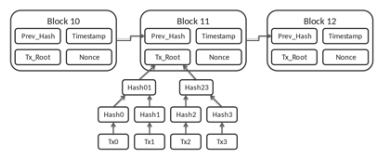
\includegraphics[width = .7\textwidth]{images/lezione6/approccio.png}
\end{center}
In una blockchain le transazioni sono raggruppate in blocchi (di n numeri di transazioni, dove n può essere diverso da un blocco a un altro) che hanno:
\begin{itemize}
    \item Timestamp di quando il blocco è stato creato
    \item Tx\_Root è una struttura dati (merkle tree: molto efficiente capire se una transazione è contenuta o meno nel blocco) che serve per memorizzare le transazioni che stanno dentro al blocco. Ogni transazione ha un hash che la rappresenta. 
    \item Nonce: un numero
    \item Prev\_Hash: collegamento al blocco precedente tramite il suo hash
\end{itemize}
\textit{Ogni nodo partecipante ha una copia della blockchain intera.}

\subsection{Problemi}
I sistemi di cui stiamo parlando sono asincroni, difficili da gestire a causa di latenza indecidibile, sincronizzazione imprecisa del clock e nodi malevoli, tutte caratteristiche che comportano:
\begin{itemize}
    \item l'ordine di arrivo delle transazioni possono essere diversi su diversi nodi
    \item alcune transazioni potrebbero contraddirsi a vicenda
    \item nodi diversi possono costruire diversi blocchi
    \item nodi diversi possono ritrovarsi con catene diverse (non si ha consenso)
\end{itemize}

\subsection{Consenso nella blockchain}
La sfida è quindi avere per ogni nodo il consenso sui blocchi e sulla sequenza di blocchi (sulla catena).\\
L'idea principale dell'algoritmo è:
\begin{enumerate}
    \item calcoliamo l'hash di ogni transazione e di un blocco
    \item quando calcolo l'hash del blocco inserisco nella funzione di hash anche l'hash del blocco precedente
    \item si include un trucco per rendere la computazione dell'hash del blocco molto dispendiosa(processo di mining), ma molto facilmente verificabile (proof of work)
    \item  se abbiamo un certo numero di nodi che vogliono fare un lavoro li si fanno competere e c'è una ricompensa (valuta di quella blockchain) per il vincitore, che si occuperà di distribuire il blocco calcolato a tutti gli altri nodi (è come eleggere un nodo che impone il suo blocco)
\end{enumerate}
L'hash di un blocco, di fatto, è la sua firma digitale. Modificando qualcosa all'interno della catena, la catena non sarà più valida, poiché occorrerà ri-validare tutti i blocchi che seguono attraverso il mining. \\
Per controllare se gli hash delle catene sono uguali, controllo l'hash dell'ultimo blocco di ciascuna catena: se sono uguali, ho il consenso sulla catena. Se non ho consenso ho il rischio che nodi diversi abbiano catene diverse.\\\\
Perchè viene dato un lavoro difficile al miner? \\
Perchè ci vorrà del tempo per risolverlo e quindi sarà più difficile avere soluzioni contemporanee. \\
Questo "puzzle" da risolvere viene calibrato in base alla quantità e alla capacità dei miner. Deve essere un problema risolvibile con algoritmi che operano con tecniche brute force, che si può far diventare più difficile progressivamente e che abbia una certa varianza.\\
Ma qual è questo problema così difficile da risolvere?

\subsection{Hashing}
Abbiamo una funzione di hash crittografica f (SHA-256):
\begin{itemize}
    \item dove f(A) ha una lunghezza fissa (per esempio 256 bit, indipendentemente dalla lunghezza dell'input A)
    \item che è resistente alle collisioni (se A diverso B anche f(A) diverso f(B)) 
    \item dove è molto difficile trovare A a partire da f(A)
    \item dove è molto facile calcolare f(A), cioè è facile verificare dati A e B se B = f(A)
\end{itemize}


\subsection{Algoritmo PoW nella Blockchain}
Il compito del miner è trovare il Nonce tale per cui il valore dell'hash finale sia più piccolo di un certo numero, scelto in modo collettivo, affinchè il tempo di risoluzione rimanga costante nel tempo.\\
Il computer deve provare con un meccanismo di brute force tutti i Nonce fino a quando non trova quello che soddisfa i requisiti.\\
È un problema progettato per richiedere un certo lasso di tempo, in modo da diminuire al minimo la probabilità che due miner risolvano l'enigma nello stesso momento.\\
Quando un miner risolve il puzzle lo annuncia a tutti.\\
Gli altri nodi, quando ricevono un messaggio da un nodo che dice di aver risolto un blocco, se effettivamente è stato verificato, lo aggiungono alla copia locale della loro catena. \\
\begin{center}
    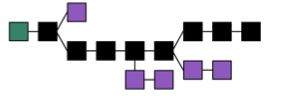
\includegraphics[width = .6\textwidth]{images/lezione6/chain.png}
\end{center}
La catena può avere dei branch (come possiamo vedere anche dalla foto), poiché siamo in una modalità concorrente, cioè i processi vengono eseguiti su nodi diversi ed è difficile prevedere chi finisce prima o dopo o quasi nello stesso momento. \\
È possibile che arrivino due blocchi entrambi validati e che abbiano lo stesso indirizzo del blocco precedente, nonostante siano diversi, formando quindi un branch.\\
La proprietà del Proof of Work fa si che ci sia una catena che si sviluppa più velocemente delle altre e che è quindi la porta ad essere la principale. \\
I blocchi che rimangono pendenti e che non fanno parte della catena prevalente, devono essere svuotati delle loro transazioni, che vengono rimesse nella pool di transazioni pending, a meno che non facciamo già parte di un blocco nella catena principale. \\
Saranno poi pescate in successivi tentativi di composizione dei blocchi.
(?) Un miner prende delle transazioni dal pool del pending, senza nessuna politica di selezione. Diversi miner possono prendere diverse transazioni. Se due miner sono al corrente di uno stesso blocco e sono d'accordo su di questo, prendono due insieme di transazioni diverse, lo risolvono e quando lo restituiscono al nodo vengono aggiunti entrambi generando il branch.(?)

\subsection{Proprietà della blockchain}
\begin{itemize}
    \item Assumendo che il maggior numero dei nodi stanno lavorando sulla stessa catena, quella che cresce più velocemente sarà la più lunga e la più veritiera.
    \item Un nodo malevolo se vuole modificare la transazione di un nodo intermedio deve anche ri-minare tutti i blocchi successivi e deve anche prevalere su tutti gli altri nodi della rete.
    \item Il meccanismo della blockchain è sicuro finchè più del 50\% del lavoro dei miner è onesto
\end{itemize}

\subsection{Limiti del Proof of Woork}
Ci sono tantissime critiche a questo algoritmo di consenso, per cui sono emerse altre proposte. \\
Non è il PoW che fa funzionare la blockchain, è l'algoritmo di consenso in generale ad essere importante.\\
I principali difetti sono:
\begin{itemize}
    \item consumo di energia e risorse (circa 1 miliardo di euro al giorno)
    \item numero di transazioni al secondo limitate
\end{itemize}

\subsection{Proof of Stake}
È detto proof-of-stake (PoS, vagamente traducibile in italiano come "prova che si ha un interesse in gioco") un tipo di protocollo per la messa in sicurezza di una rete di criptovaluta e per il conseguimento di un consenso distribuito. È basato sul principio che a ogni utente venga richiesto di dimostrare il possesso di un certo ammontare di criptovaluta. Si differenzia dai sistemi proof-of-work che sono basati su algoritmi di hash che validano le transazioni elettroniche. Peercoin è stata la prima criptovaluta ad introdurre sin dal lancio il sistema Proof of Stake senza mai implementarlo completamente. Altre note implementazioni del PoS sono BitShares, Nxt, BlackCoin e Cardano.

\subsubsection{Varianti per la selezione di un blocco}
Ogni qualvolta un nuovo blocco viene aggiunto alla blockchain, deve essere scelto il creatore del blocco successivo. Dato che quest'ultimo non può essere l'account che possiede la maggiore quantità della criptovaluta (altrimenti questo creerebbe tutti i blocchi), sono stati escogitati diversi metodi di selezione.


\paragraph{Selezione casuale (random)}
Nxt e BlackCoin utilizzano una funzione casuale per predire il generatore del blocco successivo, impiegando una formula che cerca il valore hash più basso rapportato alla dimensione della somma in gioco. Dato che la conoscenza delle somme è pubblica, ogni nodo della rete può predire - con ragionevole accuratezza - quale account si aggiudicherà il diritto di forgiare un nuovo blocco.

\paragraph{Selezione basata sull'anzianità}
La PoS di Peercoin mescola la selezione casuale con il concetto di "anzianità", un numero ottenuto tramite il prodotto del numero di monete per il numero di giorni in cui tali monete sono state possedute. Le monete che non sono state spese per almeno 30 giorni competono per la creazione del blocco successivo. Gli ammontari di monete più anziani e più grandi hanno una maggiore probabilità di firmare il blocco successivo. Eppure quando un ammontare di monete è utilizzato per firmare un blocco, questo ammontare deve ricominciare con "anzianità zero" e quindi aspettare almeno altri 30 giorni prima di poter firmare un altro blocco. E inoltre la probabilità di trovare il blocco successivo è massima dopo 90 giorni, per prevenire che somme consistenti e molto "anziane" possano dominare la blockchain. Questo processo mette in sicurezza la rete e produce gradualmente nuova valuta nel corso del tempo senza consumare una potenza computazionale significativa. Gli sviluppatori di Peercoin sostengono che questo renda più difficile attaccare la rete dato che cade il bisogno di piattaforme centralizzate di mining e inoltre acquistare più di metà delle monete è probabilmente più costoso che acquisire il 51\% della potenza di hashing della proof-of-work.

\paragraph{Selezione basata sulla velocità}
Il concetto di PoS di Reddcoin basata sulla velocità rivendica di incoraggiare la movimentazione di moneta piuttosto che il suo accumulo.

\paragraph{Selezione basata sul voto}
Invece di utilizzare solamente il concetto di posta in gioco (stake), i creatori dei blocchi possono essere selezionati mediante votazione. BitShares utilizza un sistema che comprende 101 delegati e sceglie casualmente tra essi.[1] Il voto della comunità aumenta l'incentivo dei creatori dei blocchi ad agire responsabilmente, ma al contempo apre alla prospettiva di scenari di sybil attack - come ad esempio nell'eventualità che un singolo utente impersoni i primi cinque delegati.

\subsection{Raft}
Raft è algoritmo per il consenso che è stato progettato per essere facile da capire. È l'equivante a Paxos a livello di fault-tolerance e performance.\\
Questo protocollo scompone il codice in sottoproblemi relativamente indipendenti tra loro e affronta ogni “pezzo” singolarmente.\\
Lo scopo principale di Raft è quello di rendere il consenso disponibile ad un pubblico sempre più vasto e che quest’ultimo sarà in grado di sviluppare nuovi sistemi basati sul consenso.\\
Raft si occupa della replica dei log. Intuitivamente, se si riesce a far apparire la stessa identica sequenza di log sulla maggior parte delle macchine, si è riusciti a far sì che quel cluster di macchine concordi su qualcosa.\\
In effetti, questo è chiamato trasmissione dell'ordine totale.\\ Se si riesce a far apparire ogni voce del log nella stessa posizione in un cluster di macchine, si può usarlo per implementare il consenso. \\
Ad esempio, se una macchina vuole proporre un valore e supponiamo che la sua ultima voce di registro sia nella posizione i, può provare a far sì che altre macchine mettano questo nuovo valore in i + 1 . Dopo che la maggior parte delle macchine nel cluster ha replicato quel valore in i + 1 , ora chiamiamo quel valore impegnato in i + 1 . Questo è effettivamente lo stesso che proporre un valore e farlo accettare da altri nei termini di Paxos.\\
Raft è un protocollo basato su leader. Nel suo normale corso operativo, un solo leader sarà eletto dal cluster di nodi. Gli altri nodi sono seguaci. Il leader accetta le richieste di scrittura del cliente e le replica ai follower.\\
Se si vogliono avere informazioni più approfondite su Raft si può leggere
\href{https://ichi.pro/it/protocollo-raft-consensus-reso-piu-semplice-160718622511489}{questo articolo} che ne spiega in dettaglio il funzionamento.


\subsection{Smart Contracts}
La blockchain è utile per salvare cose che vanno oltre a transazioni finanziarie. Ad esempio Ethereum è stata progettata per gli smart contracts.\\
Gli smart contract sono porzioni di codice software definiti come contratti self-executing.\\Sebbene originariamente sono stati proposti come versione digitale di contratti legali, possono essere dei programmi software generali.\\
Ogni contratto è salvato nella blockchain, diventando così immutabile.\\
Ogni nodo può verificare se le condizioni del contratto sono soddisfatte e eseguire determinate azioni (l'output deve essere validato in maniera distribuita). Alla fine tutti i nodi devono essere d'accordo sullo "stato" risultante.\\
Un esempio di applicazione potrebbe essere una piattaforma di crowdfounding senza autorità centrale.

\subsection{Permissionless vs Permissioned DLT}
Le blockchain di Bitcoin ed Ethereum sono chiamate permissionless poichè:
\begin{itemize}
    \item si ha un DL decentralizzato che traccia tutte le transazioni
    \item non ci sono terze parti fidate
    \item si ha accesso incondizionato al ledger
    \item si ha la validazione delle transazioni e la generazione di nuove monete da parte dei miners
    \item si ha la pseudo-anonimità dei partecipanti
    \item le transazioni sono immutabili
\end{itemize}
Esistono anche DLT permissioned, che vengono sfruttate soprattutto in ambito business dove ci sono molte istituzioni che usano questo meccanismo in un insieme trust limitato.\\
In queste DLT:
\begin{itemize}
    \item si ha un DL decentralizzato che traccia tutte le transazioni
    \item ci sono una o più terze parti fidate
    \item si ha un accesso condizionato al ledger
    \item  si ha la validazione delle transazioni e la generazione di nuove monete da parte dei miners
    \item si conosce l'identità dei partecipanti
    \item le transazioni sono immutabili
\end{itemize}

\subsubsection{Hyperledger Fabric}
Hyperledger nasce nel 2015 come consorzio di industrie che ha lo scopo di sviluppare una blockchain open-source per il business, hostata da Linux Foundation.\\
Fabric è uno dei sottoprogetti, originariamente gestito da IBM) che prevedeva:
\begin{itemize}
    \item permissioned DLT
    \item architettura modulare in grado di adattarsi a diversi requisiti: transazioni private, contratti confidenziali, diversi protocolli di consenso
    \item app (contratti) distribuite in linguaggi di programmazione generici
    \item nessuna dipendenza da criptovalute native
\end{itemize}



\begin{comment}
ociredeF


==============

ramO

Il problema del consenso è uno dei problemi fondamentali nel blockchain.
Nell'ambito business è considerata una tecnologia essenziale.
Nasce dalla nascita di bitcoin in avanti. Gli algoritmi che stanno alla base del paper che ha introdotto il bitcoin sono antecedenti. Il creatore di bitcoin lo ha ideato prendendo sputo da ricerca nei sistemi distribuiti. Questo whitepaper apparso nel 2008 è stato rivoluzionario. Firmato da uno pseudonimo, di cui ancora oggi non sappiamo il nome. 
Bitcoin: p2p cash system
Un mese prima dall'uscita del paper qualcuno ha registrato il nome Bitcoin, intuendo che avrebbe potuto rivoluzionre l'ambito finanziario.
Nel 2009 esce una prima implementazione di questo sistema open source. Da lì varie altre implementazioni e varianti. Questo meccanismo non va bene solo per denaro elettronico, ma ha potenziai applicazioni in molti altri ambiti. Potrebbe addirittura essere la base per avere applicazioni trusted distribuite, il cui output è trusted nonostante possano essere eseguite anche da nodi malevoli.

Nel 2013 nasce Ethereum e poi tante altre DLT.

La caratteristica di blockchain è che implementa un specie di registro delle cose che avvengono (ad esempio il registro delle transazioni immobiliari/catasto) che è immutabile (si può osservare tutta la storia). La novità è la distribuzione, non c'è un "catasto"/database(?) centralizzato che memorizza i dati, bensì è distribuito. L'obbiettivo è rendere storica l'informazione, immutabile (posso solo aggiungere e non posso cancellare), distribuita e fault tolerant (non soltanto crash, ma anche bizantine, poiché non ho fiducia in alcuni nodi che partecipano).

Le applicazioni della blockchain sono ampie. Dai quadri ai videogiochi, etc.

Il DLT System Model è un sistema distribuito. Ha un controllo decentralizzato, in cui ogni nodo esegue lo stesso codice e non c'è un controllore vero e proprio. Questi nodi sono gestiti da entità separate, non c'è un comune amministratore, e non si fidano gli uni degli altri (anche se ci sono DLT con assunzioni di trust). Dunque questo distribuito ha potenzialmente nodi con comportamento bizantino. Mettiamo una copia di tutto dappertutto. Tutti hanno una copia di questo "catasto".
Il problema del consenso, in questo caso, è che i nodi devono essere d'accordo, non sull'ultimo dato memorizzato, bensì sulla storia dei dati. 
Una blockchain è una sequenza storica di transazioni. Una transazione è un record di dati (in generale, dopodiché, essendo stata proposta in ambito finanziario ...).
Una transazione per convenzione deve avere stesso input e stesso output. Non si memorizza mai il saldo, bensì le entrate (?).

Ogni transazione che viene inserita viene firmata. Questa transazione firmata viene mandata a tutti i nodi della blockchain, perché la stessa informazione deve essere memorizzata da tutti. Nella blockchain si è identificati dalla coppia chiave pubblica/privata (se ne possono avere molte e quindi identità blockchain diverse). Quando un nodo riceve una transazione sa che arriva da un certo indirizzo blockchain. Nella transazione c'è anche la ciave pubblica del mittente in modo da fare verifiche ulteriori. C'è quindi un meccanismo di crittografia che garantisce l'origine.
Quando un nodo riceve la transazione, la valida. Come questo avviene fatto dipende dal tipo di applicazione. Bitcoin controlla dallo storico se aveva soldi dallo storico (?). Dopodiché la mette in un pool di transazioni pending. 
Da questo insieme di transazioni pending, si raggruppano in un blocco (non tutti i blocchi hanno stesso numero di transazioni). Questo blocco ha un timestamp (non necessariamente lo stesso di tutte le transazioni che sono dentro). Timestamp di quando ho fatto il blocco, non di quando ciascuna transazione è stata inserita.
ESEMPIO
Il blocco 11 contiene 4 tranazioni. Sono alla base dell'albero da Tx0 a Tx3. Sono organizzate in una struttura dati Merkle Tree, una struttura dati particolarmente efficiente per una determinata operazione. Queste transazioni hanno un corrispondente valore di hash. Abbiamo quindi una funzione di hash. Questa struttura dati è molto efficiente per capire se una transazione è contenuta oppure no nel blocco guardando l'hashing della radice. C'è inoltre un timestamp, un numero (nonce) e un "puntatore" contente un valore digitale che rappresenta il blocco precedente della catena. La cosa importante è che ognugno dei nodi ha un copia di questa blockchain. 
Blocchi e tranaszioni potrebbero avere timestamp diversi in diversi nodi, non avendo sincronizzazione perfetta. 
I problemi sono dovuti al fatto che i sistemi di cui stiamo parlando sono sistemi asincroni. Si possono fare assunzioni e accettare che qualcosa vada male, controllando poi che cosa va male. 
Problemi che in alcuni casi sono impossibili da risolvere in modo perfetto.
- La propagazione non arriva nello stesso ordine a tutti. 
- Transazioni possono essere contraddittorie
- Se le transazioni pending vengono accumulate da ogni nodo, posso avere che due nodi fanno blocchi diversi contemporaneamente.
- Possono avere catene diverse. Tutti devono avere stessa catena (problema del consenso).

L'idea dell'algoritmo proof of work è:
- calcoliamo l'hash di ciascun transazione, che da un valore come output che rappresenta quell'oggetto
- calcolo l'hash del blocco, inserendo nella funzione di hash del blocco l'identità del blocco precedente nella catena
- I nodi che calcolano l'ash del blocco devono fare un lavoro significativo (non tutti i nodi della blockchain lo fanno) chiamato mining. Alcuni dei nodi si rendono volontari di fare questo lavoro di calcolare l'hash secondo un certo trucco che è stato inserito. Chi guarda il lavoro fatto, immediatamente capisce se è fatto bene o male. Costoso da svolgere, ma immediatamente verificabile.
- Se abbiamo un certo numero di nodi (miner) che vogliono fare il lavoro, li facciamo competere. C'è un ricompensa in termini di valuta della blockchain. Si vuole eleggere quello che risolve per primo l'enigma matematico. Ci vuole anche un meccanismo per far sì che sia imrobabile (ma non impossibile) che due risolvano il problema nello stesso istante.
Diamo a ciascun miner un compito difficile in modo che ci debba mettere del tempo e sia molto improbabile che lo risolvano nello stesso momento. Questo puzzle viene calibrato man mano che i miner aumentano la capacità di risolvere il problema. 
Deve essere un problema risolvibile con brute force, che posso far diventare più difficile progressivamente e che abbia una certa varianza.

Abbiamo una funzione di hash crittografica (es. SHA256). Voglio che il suo output non sia dipendente dall'input in termini della lunghezza della stringa. Sempre stessa lunghezza. Se lo applico a due input diversi, l'output deve essere diverso. Deve essere molto difficile ricostruire input da output. Deve essere anche molto veloce calcolare l'hash e posso verificare facilmente che dato l'input A e l'output B, B = f(A).

Demo blockchain:
Il mining consiste nel trovare un nonce tale per cui l'hash del blocco sia più piccolo di un certo numero, scelto in modo collettivo affinché il tempo di risoluzione rimanga costante nel tempo. All'interno della blockchain, ogni blocco contiene l'hash del blocco precedente. L'hash di un blocco, di fatto, è la sua firma digitale. Modificando qualcosa all'interno della catena, la catena non sarà più valida, poiché occorrerà ri-validare tutti i blocchi che seguono attraverso il mining. Per controllare se gli hash delle catene sono uguali, controllo l'hash dell'ultimo blocco di ciascuna catena. Se sono uguali, ho il consenso sulla catena. Se non ho consenso, ho il rischio che nodi diversi abbiano catene diverse (?).

Il numero di transazioni può essere diverso nei diversi blocchi.

I messaggi sono firmati, per cui diventa più semplice risolvere il problema di consenso bizantino. Devo avere almeno la maggioranza dei nodi che non hanno il comportamento bizantino (2k + 1) per falsificare la transazione (?).

Risultato rilevante è il trucchetto della PoW. Quando un miner risolve il puzzle, lo annuncia a tutti. Gli altri nodi, quando ricevono un messaggio che dice di aver risolto un blocco (viene quindi mandato blocco e hash che dimostra la risoluzione facilmente verificabile), se effettivamente è stato verificato, lo aggiunge alla copia locale della catena. La catena può avere dei branch, poiché siamo in una modalità concorrente, cioè i processi vengono eseguiti su nodi diversi ed è difficile prevedere chi finisce prima o dopo o quasi nello stesso momento. è possibile che arrivino due blocchi entrambi validati e che abbiano lo stesso indirizzo del blocco precedente, nonostante siano diversi, formando quindi un branch. La proprietà del PoW fa si che ci sia una catena che si sviluppa più velocemente delle altre e che è quindi quella condivisa da tutti. I blocchi che rimangono pendenti e che non fanno parte della catena prevalente, deve rimettere le transazioni che erano in questo blocco nella pool di pending, a meno che non facciamo già parte di un blocco nella catena. Saranno pescate in successivi tentativi di composizione dei blocchi.

Un miner prende delle transazioni dal pool del pending, però non c'è una politica di selezione. Diversi miner possono prendere diverse transazioni. Se due miner sono al corrente di uno stesso blocco e sono d'accordo su di questo, prendono due insieme di transazioni diverse, lo risolvono e quando lo restituiscono al nodo vengono aggiunti entrambi generando il branch.

I miner sono anche nodi della catena.

Le proprietà che emergono sono:
- se la maggior parte dei nodi lavorano sulla stessa catena ...
- non solo, se vuole cambiare qualcosa nella catena, deve ricalcolare i blocchi, ma deve anche imporsi sulla catena più lunga (?).
- più del 50\% del lavoro dei miner deve essere onesto

Ci sono tantissime critiche a questo algoritmo di consenso, per cui sono emerse altre proposte. Non è il PoW che fa funzionare la blockchain, è l'algoritmo di consenso in generale ad essere importante.

L'elettricità costa parecchio per fare PoW (1 miliardo al giorno) e le transazioni sono poche.

Il consenso non c'è mai sull'ultimo blocco soltanto, ma dev'essere sulla storia della catena.

Sono stati proposti diversi algoritmi di consenso, ad esempio Raft, algoritmo di consenso per altro tipo di blockchain: permissioned (?).
Proof of stake sostiene che chi ha più potere/risorse decide quale blocco aggiungere. In più c'è un meccanismo randomico, non c'è la selezione esatta di chi ha più risorse. Inoltre c'è il discorso dell'età: da quanto tempo questo verificatore del blocco fa parte della blockchain? Più è alto è il tempo, più è alta la fiducia. L'intuizione dietro a questa scelta è che il danno che loro avrebbero nell'essere malevoli nella blockchain è superiore al guadagno. Quando uno di questi volontari viene scelto, il suo account viene congelato fino a quando non si capisce che la validazione è stata corretta e dopodiché viene rilasciato.

In Raft viene fatta un'elezione in modo distribuito. Non sempre è l'id maggiore che vince, poiché questo può essere costruito per esempio guardando quanti soldi hanno nel conto e far emergere quello che ha più soldi. Bisogna escludere quello dal comportamento malevolo, poiché si è deciso di farlo in termini di fiducia. Se il validatore cerca di compromettere il sistema/validare transazioni fraudolenti dentro al blocco, perdono tutto.

Come si previene il double spending problem? (uso i miei soldi per due transazioni cercando di comprare due cose con gli stessi soldi)
VIDEO

Nel 2012-13 è apparso un articolo che propone una generalizzazione dell'uso di blockchain, rendendo esplicita la cosa. Da qui nasce Ethereum, che generalizza, rispetto a transazioni finanziarie, a smart contract (più eterogenea) e ha un suo linguaggio per scrivere gli smart contract.

Queste blockchain vengono chiamate permissionless: chiunque può decidere di partecipare e vedere le transazioni dentro la blockchain. C'è pseudoanonimità dei partecipanti. 

Ci sono anche DLT permissioned. Soprattutto in ambito business ci sono molte istituzioni che usano questo meccanismo tra un insieme di aziende (trust limitato). Limitare la partecipazione e aggiungere un controllo. Abbiamo identità nota dei partecipati. Ci sono delle identità trusted. Ci sono anche qui criptovalute legate a questo. Una di queste piattaforme per la generazione di DLT è hyperledger, in particolare hyperledger fabric (inizialmente fatto da IBM e poi ceduto). È possibile sviluppare gli smart contract (in ethereum c'è un linguaggio apposta) con general purpose programming languages, posso quindi scrivere codice all'interno dei dati che vengono racchiusi in blocchi.

------------
Fabbio
DLT: tecnologie blockchain

Nell'ambito business la blockchain è considerata una tecnologia essenziale. 
Storia:
Nel 2008 nasce un paper firmato da satoshi nakamoto (pseudonimo) intitolato Bitcoin. Bitcoin è un peer-to-peer cash system. Il mese prima dall'uscita del paper qualcuno aveva registrato il nome Bitcoin.
Nel 2009 esce la prima implementazione opensource e da lì in poi varie implementazioni e varianti.
Il meccanismo ha potenziali applicazioni in moltissimi ambiti. Potrebbe essere la base per avere applicazioni distribuite trusted il cui output è trusted nonostante possano essere eseguite anche da nodi malevoli.

nel 2013 esce ETH e via...

La caratteristica di blockchain che ispira altre applicazioni oltre al denaro elettronico è che implementa un registro delle cose che avvengono (tipo registro transazioni immobiliari o catasto immobiliare..). 
A differenza dei database il "catasto" viene distribuito su vari nodi. L'obiettivo è rendere storica, immutabile e full tolerance l'informazione.


Il modello del sistema DLT
-E' un sistema distribuito
-Ha un controllo decentralizzato in cui non c'è un coordinatore e ogni nodo esegue lo stesso codice
-I nodi sono gestiti da entità separate e non si fidano gli uni degli altri
Dunque il sistema distribuito ha assumibilmente nodi con comportamento "bizzantino"

Problema del consenso:
I nodi devono essere d'accordo su di uno storico dei dati. I nodi devono essere d'accordo sulla storia dei dati.

DATI NELLA BLOCKCHAIN
Una blockchain è una sequenza storica di transazioni
Transazione: Record di dati. Nell'ambito finanziario [A trasferisce x a B]
Una transazione per convenzione deve avere lo stesso input e lo stesso output.

L'APPROCCIO BLOCKCHAIN
Ogni transazione inserita viene firmata. Si utilizza il meccanismo di chiavi asimmetriche e ogni partecipante ha una chiave privata e una pubblica. Quando una transazione viene firmata, questa viene mandata a tutti i nodi della blockchain.
Quando un nodo riceve una transazione sa da quale nodo arriva. 
Nel codice condiviso che tutti i nodi hanno, c'è una porzione che dice "Quando arriva una transazione validala". Dunque il nodo che riceve va a vedere nello storico se la transazione è plausibile. 
Dunque: A mette una tranazione nel sistema che va a tutti i nodi. Chi la riceve guarda nello storico se è valida. Poi la mette in un pool di transazioni pending.
QUANDO PASSA IN UNO STATO APPROVED?

APPROCCIO BLOCKCHAIN:
Dall'insieme di transazioni pending, si raggruppano in un blocco (non tutti i blocchi hanno lo stesso numero di transazioni), il blocco ha un timestamp che non è lo stesso di tutte le transazioni che ha al suo interno. Nel blocco X (11 nelle slide) c'è il TX room: struttura dati per memorizzare le transazioni nel blocco. Ogni transazione ha il corrispondente valore di hash e la struttura dati ha la particolarità che è molto efficiente capire se una transazione è avvenuta o no.
C'è un certro numero di transazioni nel blocco e c'è una funzione per capire molto velocemente se all'interno del blocco c'è o meno la transazioni.
Da un blocco all'altro si collegano tramite un puntatore (valore digitale del blocco precedente viene scritto nel blocco successivo e viceversa). 
Ognuno dei nodi ha la copia di questa blockchain.

PROBLEMI:
I blocchi e le transazioni potrebbero avere timestamp diversi su diversi nodi. 
I problemi sono dovuti al fatto che i sistemi sono asincroni dove possono capitare le cose più bizzarre. Alcune transazioni potrebbero essere contraddittorie. Nodi diversi potrebbero creare blocchi diversi. Tutti i nodi devono avere la stessa blockchain. (Problema del consenso)

CONSENSO DELLA BLOCKCHAIN
Idea: si calcola l'hash di ogni transazione che da in output un certo valore che rappresenta l'oggetto. Calcolo l'hash del blocco. Quando calcolo l'hash del blocco inserisco l'identità digitale del blocco precedente e ci includo...
Non tutti i nodi della blockchain fanno il lavoro del calcolo dell'hash, e questo lavoro viene fatto dai miners. I miners introducono nella blockchain nuova valuta.
Alcuni dei nodi dunque si rendono volontari per calcolare l'hash con un trucco particolare. Il lavoro è duro e costoso ma immediatamente verificabile. (Idea dietro l'algoritmo di consenso)
Se si hanno un certo numero di nodi che vogliono minare, li si fa competere su di un blocco. C'è un compenso nella valuta della blockchain. Diversi nodi dunque si mettono a validare un blocco è tra tutti questi bisogna sceglierne uno. Quello che si elegge è quello che risolve prima "l'enigma matematico". Ci può essere il caso in cui 2 riescono risolvere il puzzle allo stesso momento.

PROBLEMI DIFFICILI:
perchè deve essere difficile? Perchè devono metterci tempo così che tutti finiscano in tempi differenti. La difficoltà del puzzle viene aumentata in base alla capacità del miner di risolvere il problema. Il problema deve essere un problema che dal punto di vista computazionale viene risolto in bruteforce, può avere una certa varianza (puoi essere fortunato o sfortunato a risolverlo).
Statisticamente è più difficile che più miners lo risolvono a diversi istanti.

QUAL è QUESTO PROBLEMA?
Funzione di Hashing crittografica con proprietà tipo:
Output indipendente dalla lunghezza dell'input.
Deve essere collision resistent.
Dallì'output deve essere quasi impossibile risalire all'input.
Deve essere facile da verificare.

PROPRIETA' BLOCKCHAIN:
La catena che cresce più velocemente sarà quella che merita fiducia. 


\end{comment}
\chapter{Sviluppo}
\lhead{Sviluppo - Mobile Computing}
\begin{center}
    \textbf{--------- Lezione 7 - 25 marzo 2021 ---------}
\end{center}

\section{Panoramica}
Le due librerie principali per lo sviluppo di applicazioni AR sono:
\begin{itemize}
    \item ARKit di Apple: è utilizzabile sui device mobili Apple recenti e non utilizzabile su simulatore
    \item ARCore di Google: può essere utilizzata in nativo su Android ed è utilizzabile, con alcune limitazioni, su simulatore
\end{itemize}
\subsection{Macro funzionalità}
Per realizzare applicazioni in realtà aumentata, ARKit e ARCore forniscono funzionalità per semplificare le seguenti operazioni:
\begin{itemize}
    \item Registration e Tracking
    \item Scene
    \item Display
    \item Interaction
\end{itemize}

ARKit e ARCore condividono alcuni concetti base:
\begin{itemize}
    \item scene (ARKit) / session (ARCore): due nomi diversi per lo stesso concetto, che rappresenta l'ambiente rispetto al quale effettuiamo la registration. Gli oggetti virtuali e reali sono posizionati nel sistema di riferimento della scena/sessione. Fornisce le chiamate per accedere agli altri elementi di AR
    \item configuration: definisce le caratteristiche della scena / sessione da creare:
    \begin{itemize}
        \item rispetto a cosa facciamo la registration, ad esempio rispetto all'ambiente 3D circostante, viene creato un sistema di riferimento in una posizione iniziale e si tiene traccia dello spostamento rispetto a questo sistema
        \item rispetto a cosa siamo interessati a riconoscere
    \end{itemize}
    \item ancore: rappresentano dei punti di riferimento agli oggetti virtuali o reali identificati. Es: quando un oggetto viene riconosciuto, viene associato ad un’ancora. Attraverso l’ancora possiamo risalire alla posizione e rotazione (6DOF) dell'oggetto rispetto alla scena. Le ancore si usano ad esempio quando riconosciamo i piani ed ogni piano è rappresentato dalla propria ancora
    \item hitTest/rayCasting: si tratta di un’operazione per convertire le coordinate schermo (2D) in un punto 3D. Concettualmente devo considerare il raggio, che “esce” dal device verso lo spazio, che interseca zero o più oggetti (reali o virtuali) ed hitTest ritorna l’insieme di questi oggetti
\end{itemize} 

\subsection{Comprendere la scena}
ARKit e ARCore forniscono alcuni strumenti che semplificano il processo di comprensione della scena:
\begin{itemize}
    \item riconoscimento piani
    \item riconoscimento immagini (2D): la procedura avviene in 3 passi:
        \begin{itemize}
            \item aggiunta dell'immagine alle risorse del progetto: si fornisce ad ARKit/ARCore l'immagine da riconoscere e la dimensione attesa nel mondo reale
            \item modifica della configurazione della scena, indicando, da codice, che si vuole riconoscere quell'immagine
            \item specificare cosa fare quando l'immagine viene riconosciuta: si gestisce l'evento di quando l'ancora relativa a quell'immagine viene aggiunta
        \end{itemize}
    \item riconoscimento dei volti
    \item riconoscimento oggetti (3D): dobbiamo prima ottenere un modello 3D dell'oggetto e poi il procedimento di riconoscimento è analogo a quanto avviene per le immagini 2D 
\end{itemize}

\section{Alcune funzionalità di ARKit 4}
\subsection{AR multiuser}
Sia in ARKit che in ARCore si possono avere più scene/sessioni condivise tra più utenti. 
Prendiamo ad esempio un utente identifica dei feature point e poi si identifica tramite l'ambiente. Se quelle stesse informazioni vengono condivise con un altro utente e il device di questo, riesce a capire dove si trova rispetto ai fp del primo utente, possiamo fare la registrazione rispetto ad un sistema di riferimento comune. Questo permette di mostrare un oggetto virtuale nello stesso punto a diversi utenti con diverse angolazioni. 
\begin{center}
    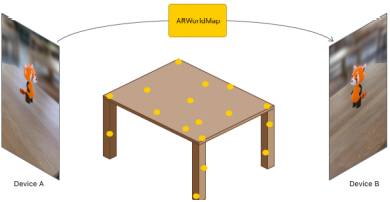
\includegraphics[width=.7\textwidth]{images/MobiDEV/5. augmented reality in pratica/ar multiuser.PNG}
\end{center}

\subsection{Scene geometry}
I device che hanno un sensore di profondità (Lidar) possono creare una ricostruzione topologica dell'ambiente. La libreria AR per i dispositivi con Lidar mette a disposizione funzionalità per:
\begin{itemize}
    \item riconoscere gli oggetti
    \item calcolare quando un oggetto si interpone tra la camera e un oggetto virtuale, così da risolvere il problema dell'occlusione
    \item permettere agli oggetti virtuali di rispettare alcune regole della fisica nell'interazione con oggetti del mondo reale (ad esempio due oggetti che non si possono compenetrare)
\end{itemize} 
Attraverso il lidar è anche possibile andare a creare una configurazione chiamata body tracking dove il sistema riconosce le principali articolazioni del corpo e ce le restituisce come nodi, ovvero punti che possiamo tracciare, cosicché possiamo calcolare la posizione del corpo e come si muove l'utente. Questa procedura si chiama \textbf{Motion capture}.
\chapter{Testing e debugging}
\lhead{Testing e debugging - Mobile Computing}
\begin{center}
    \textbf{--------- Lezione 8 - 21 ottobre 2020 ---------}
\end{center}

\section{Approccio alla scrittura del codice}
La scrittura di un programma di un sistema complesso passa attraverso una serie di errori. 

Uno degli errori più comuni è scrivere tutto o buona parte del codice e poi verificare se l'effetto finale del software realizzato è quello desiderato. 
Il problema è che non funziona mai al primo tentativo e correggere gli errori diventa molto complicato, perché non si sa dove possono essere.

L'idea è quella dividere il processo di sviluppo in tanti piccoli passi, ognuno dei quali può essere provato per controllarne il funzionamento. 
Più difficile è il codice che si scrive, più i passi devono essere piccoli. Anche una sola riga di codice, se ad esempio si sta usando una tecnologia che non si conosce bene. 

Il problema è che, a volte, abbiamo delle righe di codice che non producono un effetto visibile, come la gestione degli eventi. 
Per questo bisogna scrivere del codice per verificare lo stato di un'applicazione, come l'utilizzo di messaggi di log.

Il tempo di sviluppo è in buona parte dedicato a correggere gli errori soprattutto quando lo sviluppatore è inesperto che scrive tutto il codice insieme. 
Ridurre il numero di errori e il tempo necessario per correggerli è 
l’obiettivo principale se si vuole sviluppare velocemente.

Dividere il codice in piccole parti verificabili è difficile. 
Prima di iniziare a sviluppare una parte di codice bisogna pensare a come suddividerla in parti, sfruttando l'utilizzo di carta e penna, o di algoritmi in pseudo codice. 
Un errore comune è che viene provata l'app senza sapere cosa aspettarsi. Prima di fare una prova bisogna pensare a cosa ci si aspetta che sia il risultato.

Diverse parti del codice vengono adattate da esempi trovati online. Questi sono i casi nei quali è più facile commettere errori, perché magari non conosciamo esattamente le operazioni che fa il codice. 

Due strategie di sviluppo sono:
\begin{itemize}
    \item top-down: iniziare a scrivere le funzioni principali per poi scrivere i metodi di dettaglio che sono necessari per le funzioni principali
    \item bottom-up: iniziare a scrivere i metodi di dettaglio per poi comporli nelle funzioni principali
\end{itemize}

Prendiamo ad esempio un algoritmo di ordinamento di un array composto da due funzioni:
\begin{itemize}
    \item la funzione principale di ordinamento
    \item la funzione che scambia il valore di due elementi dell'array
\end{itemize}
Nell'approccio top-down prima viene scritta la funzione principale di ordinamento, poi quella che scambia i due valori

Nell'approccio bottom-up prima viene scritta la funzione che scambia i due valori, poi quella di ordinamento.

Nella programmazione tipicamente si usa una combinazione di approccio bottom-up e top-down.

%%%%%%%%%%%%% inizio esempio di algoritmo passo passo %%%%%%%%%%%%%
\begin{comment}

\subsection{Esempio: definizione e problema}
Abbiamo un array che contiene tutte le parole scambiate in 10.000 conversazioni su un sistema di chat. Ogni elemento dell'array è una singola parola. 
L'obiettivo è scrivere un metodo per trovare quante volte occorre una data parola. 

\begin{Java}
    //codice
    ArrayList<String> = wordsArray = ...
    //altro codice
    int a = wordCount(wordsArray, "ciao"); 
    //stampa del valore di a
\end{Java}
\newpage
La prima operazione è quella di ideare la procedura e scrivere il procedimento che risolve il problema: \\
input: array di parole e una parola \\
Output: il numero di volte che la \\
parola occorre nell’array \\
Procedura: \\
- Inizializzo un contatore a zero \\
- Scorro tutte le parole \\
dell'array \\


Poi possiamo procedere a convertire l'algoritmo in codice passo dopo passo:
\begin{itemize}
    \item passo 1: creo un metodo che ritorna sempre lo stesso valore
    \begin{Java}
        private int wordsCount(ArrayList<String> words,
                                String target) {
            return 0;
        }   
    \end{Java}
    \item passo 2: inizializzo e ritorno il contatore
    \begin{Java}
        private int wordsCount(ArrayList<String> words,
                                String target) {
            int counter = 0;
            return counter;
        }   
    \end{Java}
    \item passo 3: verifico di saper scrivere un codice che scorre tutti gli elementi
    \begin{Java}
        private int wordsCount(ArrayList<String> words,
                                String target) {
            int counter = 0;
            for(String word:words){
                counter++;
            }
            return counter;
        }   
    \end{Java}
    \item passo 4: verifico di saper controllare se la prima parola dell’array è quella cercata
    \begin{Java}
        private int wordsCount(ArrayList<String> words,
                                String target) {
            int counter = 0;
            String word = words.get(0);
            if (word.equalsIgnoreCase(target))
                counter++;
            return counter;
        }   
    \end{Java}  
    \item passo 5: metto assieme i due passi precedenti 
    \begin{Java}
        private int wordsCount(ArrayList<String> words,
                                String target) {
            int counter = 0;
            for(String word:words){
                if (word.equalsIgnoreCase(target))
                counter++;
            }
            return counter;
        }   
    \end{Java} 
\end{itemize}
\end{comment}
%%%%%%%%%%%%% fine esempio di algoritmo passo passo %%%%%%%%%%%%%
\section{Testing}
Il testing di un'app ha lo scopo di valutare diversi aspetti:
\begin{itemize}
    \item funzionalità: l'applicazione fa quello che dovrebbe?
    \item usabilità: l'utente riesce ad usare l'app come previsto?
    \item performance: l'applicazione ha le performance desiderate?
    \item sicurezza: l'app è soggetta ad attacchi di sicurezza o privacy?
\end{itemize}

Se emergono problemi durante il testing significa che l'operazione è efficace. 
Se non emergono problemi in fase di test l'applicazione è corretta oppure non sono stati svolti i test corretti. 

Il testing sui dispositivi mobili ha diverse peculiarità: 
\begin{itemize}
    \item i dispositivi sono diversi dal punto di vista hw e sw
    \item diversi contesti di utilizzo: c'è connessione ad internet? potrebbe essere molto rallentata? i server a cui l'app si connette funzionano o sono molto lenti? ecc.
    \item interrupt che avvengono durante l'uso
    \item il codice su dispositivi mobili è basato su eventi. La sequenza con cui avvengono gli eventi spesso non è deterministica e di fatto si pongono dei problemi di concorrenza
\end{itemize}

Il fatto che l’applicazione funzioni una volta non significa che sia corretta perché potrebbe presentare degli errori in futuro, anche se eseguita nello stesso modo sullo stesso HW, SW, nello stesso contesto e con gli stessi interrupt.

Per effettuare un test di un'applicazione concorrente, dobbiamo provare tutte le possibili combinazioni di ordine di chiamate.
Questo però è un problema, perché provare tutte le combinazioni  per ogni device in commercio, è impossibile.

Al posto che svolgere tutti i test per tutti i possibili casi, ciascun test si svolge solo in alcuni caso. In questo modo si hanno meno casi, ma è possibile che qualche caso problematico sia tralasciato. 
\\ Linee guida e best practice da utilizzare:
\begin{itemize}
    \item scegliere i dispositivi più diffusi e caratteristici, tipicamente almeno 2 smartphone e 2 tablet
    \item svolgere i test con la versione minima supportata del SO e uno con la versione più recente
    \item svolgere i test in assenza di problemi e in presenza dei problemi più comuni come la mancanza o il rallentamento della connessione
    \item verificare il funzionamento di tutto il codice
    \item provare l'app su dispositivi diversi
    \item provare l'app in situazioni particolari come assenza o rallentamento della connessione Internet
\end{itemize}

Fare il test di un’applicazione è un’operazione lunga, soggetta ad 
errori che deve essere fatta ogni volta che si mette mano al codice. L'idea è quella di automatizzare il test. 

Alcuni parti possono essere automatizzate, scrivendo del codice che verifica la correttezza di altre parti del codice. 
\\ Questo codice può, ad esempio, creare istanze delle classi del model o generare degli eventi su oggetti di interfaccia. 

Esistono diverse librerie che supportano i test automatizzati. I test automatizzati hanno una chiamata "assert" che indica cosa ci si aspetta sia vero. 
Se tutti gli assert sono verificati, il test ha successo, altrimenti fallisce.
\\ Un esempio ne è il testing del model: viene creata un'istanza della classe che si vuole testare, si richiama il metodo e si verifica, attraverso un assert, che il risultato del metodo sia quello che atteso.
 
Un altro esempio è il testing della view-controller: ci sono librerie che permettono di scrivere del codice al cui interno si possono scatenare degli eventi sugli oggetti interfaccia, ovvero simulare un'azione che farebbe un utente e si verifica che il risultato sia quello atteso.

\subsection{Pro e contro dell'automazione del testing}
Il vantaggio del testing è che dopo aver scritto il codice di test, il test avviene molto velocemente. 
La scrittura di test, però, è onerosa ed è soggetto ad errori: può segnalare errori che non ci sono o ignorare errori che ci sono. 

In generale il test automatizzato è molto vantaggioso per progetti che devono essere mantenuti nel tempo, cioè quasi tutti i progetti commerciali, mentre nei prototipi a volte potrebbe essere controproducente. 

Si può verificare il comportamento delle singole componenti attraverso unit testing. 

\section{Debugging}
Il debugging funziona meglio se combinato con una procedura di scrittura passo passo. 
Il debugging è la procedura attraverso la quale si identifica e risolve un bug, cioè un problema che causa un malfunzionamento.

Si divide in tre passi principali:
\begin{itemize}
    \item riprodurre il malfunzionamento: per algoritmi deterministici è semplice, lo stesso input produce sempre lo stesso output deterministico, ma in realtà in casi pratici non è così. Se si effettua un test manuale (non automatizzato) bisogna trovare una serie di passaggi che generino sempre l'errore: se i passaggi sono lunghi da riprodurre, è conveniente modificare temporaneamente il codice per velocizzare il test
    \item trovare il bug: vengono usati due strumenti principali: logging e debugging. È possibile eseguire un'applicazione in modalità debugging: l'esecuzione si ferma in alcuni punti definiti dal programmatore
    \item risolvere il bug: ci sono varie strategie per trovare e risolvere gli errori:
    \begin{itemize}
        \item "piccoli passi"
        \item tecnica "wolf fence": ricerca dicotomica
        \item "torna indietro e prova": cancello delle righe commentando fino a quando non arrivo ad una riga in cui il codice funziona. Pian piano si decommenta
        \item "semplifica il codice": se il bug si verifica in una riga di codice, ma è complicata. Si può riscrivere la riga di codice in più righe e andare a verificarle una dopo l'altra
    \end{itemize}
\end{itemize}

\subsection{Logging}
Una parte del codice dell'applicazione può essere finalizzata a stampare messaggi per il programmatore, così che possa capire meglio cosa accade nel codice. I log, a volte, vengono inseriti ancora prima di avere un bug, perché servono anche da documentazione del codice.
In Android abbiamo accesso a tutti i log del sistema e il problema è che il nostro messaggio vada perso tra tutti gli altri. 
È possibile filtrare i messaggi di log per:
\begin{itemize}
    \item processo: spesso selezionare il processo giusto non basta, perché ci sono tanti messaggi di log non scritti da noi, ma generati da altre componenti del nostro processo
    \item importanza: vengono mostrati tutti i messaggi più importanti del livello scelto, ma a volte non basta
    \item tag: per ogni messaggio si usa un TAG che permette di categorizzare il messaggio e un testo
\end{itemize}

\subsection{Errori comuni}
\begin{itemize}
    \item il messaggio d'errore non viene letto. In molti casi si può trovare il messaggio lungo e non sempre è semplice capirlo
    \item testare l'app senza sapere cosa aspettarsi: prima di provare l'app bisogna avere chiaro cosa ci si aspetta che l'app faccia
    \item l'app non fa ciò che dovrebbe: ad esempio va in crash
    \item fare sempre le stesse operazioni durante le prove dell'applicazione, ma si rischia di testare le stesse parti del codice
\end{itemize} 


%%%%%%%%%%% FINITO %%%%%%%%%%% 
